\documentclass[11pt,a4paper]{article}

% -----------------------------------------------------------------------------
% cnavier scientific methodology / user manual
% Repository state reviewed: main @ 5018e29bff534b252a7ac9025ece4ac43efd78ad
% Generated: 2026-10-06
% -----------------------------------------------------------------------------

\usepackage[margin=2.5cm]{geometry}
\usepackage[T1]{fontenc}
\usepackage[utf8]{inputenc}
\usepackage{lmodern}
\usepackage{microtype}
\usepackage{amsmath,amssymb,bm}
\usepackage{booktabs}
\usepackage{graphicx}
\graphicspath{{figures/}}
\usepackage{longtable}
\usepackage{array}
\usepackage{enumitem}
\usepackage{xcolor}
\usepackage{listings}
\usepackage{hyperref}
\usepackage{cleveref}

\hypersetup{
  colorlinks=true,
  linkcolor=blue!50!black,
  citecolor=blue!50!black,
  urlcolor=blue!60!black,
  pdftitle={cnavier: Numerical Methodology and Scientific User Manual}
}

\lstset{
  basicstyle=\ttfamily\small,
  frame=single,
  breaklines=true,
  columns=fullflexible,
  keepspaces=true,
  showstringspaces=false
}

\newcommand{\Rey}{\mathrm{Re}}
\newcommand{\dd}{\mathrm{d}}
\newcommand{\dt}{\Delta t}
\newcommand{\dx}{\Delta x}
\newcommand{\dy}{\Delta y}
\newcommand{\Oh}{\mathcal{O}}
\newcommand{\code}[1]{\texttt{\detokenize{#1}}}

\title{\textbf{cnavier}\\[0.5em]
\large Numerical Methodology and Scientific User Manual}
\author{cnavier project}
\date{Repository state: \code{main} at \code{5018e29bff534b252a7ac9025ece4ac43efd78ad}\\6 October 2026}

\begin{document}

\maketitle

\begin{abstract}
\texttt{cnavier} is a compact two-dimensional incompressible Navier--Stokes solver written in C, with optional OpenMP and CUDA acceleration.  The code advances the scalar vorticity equation and reconstructs a divergence-free velocity field from a stream function.  Spatial derivatives are represented by finite-difference matrices of selectable interior order (second, fourth, or sixth), assembled into two-dimensional sparse operators through Kronecker products and applied in compressed sparse row (CSR) form.  Time integration is explicit, using either forward Euler or classical fourth-order Runge--Kutta (RK4).  The stream-function Poisson equation may be solved by Gauss--Seidel, successive over-relaxation (SOR), or a direct discrete-sine-transform solver implemented with FFTW3 on the CPU and cuFFT on the GPU.

This document describes the mathematical model, the exact discretizations present in the source code, solver sequencing, boundary treatment, stability considerations, verification and validation strategy, parallel backends, usage, and current numerical limitations.  It is intended to be both a scientific description of the methodology and a practical reference for users and developers.
\end{abstract}

\tableofcontents
\newpage

% =============================================================================
\section{Introduction}
% =============================================================================

The objective of \texttt{cnavier} is to provide a small, inspectable computational fluid dynamics (CFD) code for two-dimensional incompressible viscous flow.  Its reference problem is the square lid-driven cavity: three stationary no-slip walls and one tangentially moving wall.  Despite the small code base, the project contains several numerical alternatives that are useful for study and benchmarking: multiple finite-difference stencil widths, two explicit time integrators, three elliptic solvers, a sparse-operator formulation, shared-memory parallelism, and an optional CUDA implementation of the complete time loop.

The code uses a \emph{vorticity--streamfunction} formulation rather than the primitive-variable $(u,v,p)$ equations.  This choice removes pressure from the evolution system and replaces the pressure--velocity coupling problem by a scalar Poisson equation.  In two dimensions, the streamfunction definition also gives a particularly strong discrete incompressibility property: when the discrete $x$- and $y$-derivative operators commute, the recovered velocity has zero discrete divergence to round-off.

The solver is designed primarily as an educational and experimental code rather than as a general-purpose production CFD package.  The current implementation assumes a rectangular Cartesian domain, a Cartesian computational array, constant Reynolds number, explicit time stepping, and Dirichlet wall velocities.  These constraints simplify the formulation sufficiently that each numerical operation can be followed directly from the governing equations to its C or CUDA implementation.

\subsection{Repository organization}

The main numerical components are:

\begin{itemize}[leftmargin=2em]
  \item \code{src/main.c}: run configuration, command line, operator construction, time loop, diagnostics, and output;
  \item \code{src/backend.c}: one interface over the CPU and CUDA solvers, and the choice between them;
  \item \code{src/finitediff.c}: one-dimensional first- and second-derivative finite-difference matrices, with walls or periodic, and CSR conversion;
  \item \code{src/linearalg.c}: dense storage utilities, CSR sparse matrices, sparse matrix--vector multiplication, and Kronecker products;
  \item \code{src/fluiddyn.c}: wall conditions, vorticity transport, Euler and RK4 integration, recovery of the velocity from the streamfunction, and full timesteps;
  \item \code{src/poisson.c}: Gauss--Seidel, SOR, and FFTW/DST-I Poisson solvers, and the periodic FFT solver;
  \item \code{src/cudasolver.cu}: CUDA implementations of the time loop, sparse operators, elliptic solvers, and diagnostics;
  \item \code{src/threads.c}: the default number of OpenMP threads (one per physical core);
  \item \code{src/forcing.c}: Kolmogorov and random forcing;
  \item \code{src/diagnostics.c}: energy, enstrophy and palinstrophy, and on periodic grids spectra and spectral fluxes;
  \item \code{src/utils.c}: VTK output, centerline data for comparison with Ghia et al., and the available-memory check;
  \item \code{tests/test_solver.c}: CPU verification and CPU--GPU parity tests.
\end{itemize}

% =============================================================================
\section{Governing Equations}
% =============================================================================

\subsection{Nondimensional incompressible Navier--Stokes equations}

For an incompressible Newtonian fluid of constant density and viscosity, the nondimensional two-dimensional Navier--Stokes equations are
\begin{align}
\frac{\partial \bm{u}}{\partial t}
+ (\bm{u}\cdot\nabla)\bm{u}
&= -\nabla p + \frac{1}{\Rey}\nabla^2\bm{u},
\label{eq:NS}\\
\nabla\cdot\bm{u} &= 0,
\label{eq:continuity}
\end{align}
where
\[
\bm{u}=(u,v)^T
\]
is the velocity, $p$ is the kinematic pressure, and
\[
\Rey=\frac{U_{\mathrm{ref}}L_{\mathrm{ref}}}{\nu}
\]
is the Reynolds number.

For the default lid-driven cavity, $L_{\mathrm{ref}}=1$ and the lid speed is $U_{\mathrm{ref}}=1$, so the default nondimensional boundary data are
\begin{align*}
(u,v)&=(1,0) &&\text{on the moving lid},\\
(u,v)&=(0,0) &&\text{on the other three walls}.
\end{align*}

\subsection{Vorticity--streamfunction formulation}

Define the scalar vorticity
\begin{equation}
\omega = \frac{\partial v}{\partial x}-\frac{\partial u}{\partial y}.
\label{eq:vorticity-def}
\end{equation}
Taking the curl of \cref{eq:NS} eliminates pressure and yields the vorticity transport equation
\begin{equation}
\frac{\partial \omega}{\partial t}
+u\frac{\partial\omega}{\partial x}
+v\frac{\partial\omega}{\partial y}
=\frac{1}{\Rey}\left(
\frac{\partial^2\omega}{\partial x^2}
+\frac{\partial^2\omega}{\partial y^2}
\right).
\label{eq:vort-transport}
\end{equation}

Introduce a streamfunction $\psi$ by
\begin{equation}
 u=\frac{\partial\psi}{\partial y},
 \qquad
 v=-\frac{\partial\psi}{\partial x}.
\label{eq:velocity-streamfunction}
\end{equation}
Substitution into \cref{eq:vorticity-def} gives
\begin{equation}
\nabla^2\psi=-\omega.
\label{eq:poisson}
\end{equation}
Thus a timestep consists conceptually of transporting $\omega$, solving the elliptic problem \cref{eq:poisson}, and differentiating $\psi$ to obtain the velocity.

\subsection{Why incompressibility is naturally enforced}

At the continuous level, \cref{eq:velocity-streamfunction} gives
\[
\nabla\cdot\bm{u}
=\frac{\partial^2\psi}{\partial x\partial y}
-\frac{\partial^2\psi}{\partial y\partial x}=0.
\]
The code mirrors this property discretely.  Let $D_x$ and $D_y$ denote the two-dimensional derivative matrices.  The recovered velocity is
\begin{equation}
\bm{u}_h =
\begin{bmatrix}
D_y\bm{\psi}\\
-D_x\bm{\psi}
\end{bmatrix}.
\end{equation}
The discrete divergence is therefore
\begin{equation}
D_xD_y\bm{\psi}-D_yD_x\bm{\psi}.
\end{equation}
Because the operators are built as Kronecker products acting in separate coordinate directions, they commute algebraically under the implemented layout.  Consequently, the divergence diagnostic is expected to be near machine precision, apart from floating-point effects and details of the boundary rows.  This behavior is explicitly tested by the project.

% =============================================================================
\section{Computational Grid and Data Layout}
% =============================================================================

\subsection{Domain and spacing}

The physical domain is specified by $L_x$ and $L_y$ and the computational array by $n_x\times n_y$.  The implementation defines
\begin{equation}
\dx=\frac{L_x}{n_x-1},
\qquad
\dy=\frac{L_y}{n_y-1},
\label{eq:grid-spacing}
\end{equation}
$n_x$ and $n_y$ are independent; each may range from 8 through 16384.

Fields are stored as contiguous row-major arrays wrapped by the \code{mtrx} structure, with $n_y$ rows of $n_x$ values: element $(i,j)$ lies at $y=i\,\dy$, $x=j\,\dx$ and has flat index $i\,n_x+j$, which is the ordering the Kronecker operators of \cref{eq:kron-ops} assume.  Earlier versions stored $n_x$ rows of $n_y$ values while the operators assumed the transpose; the two only agree when $n_x=n_y$, so non-square grids were rejected.  Flattening a field is therefore a direct memory copy, and the two-dimensional derivative operations are implemented as sparse matrix--vector products.

\subsection{Grid convention}

The grid is nodal.  Column $j$ lies at $x_j=j\,\dx$, $j=0,\dots,n_x-1$, and row $i$ at $y_i=i\,\dy$, $i=0,\dots,n_y-1$, so the first and last rows and columns of the arrays lie on the walls and $n_x$ nodes span $L_x$ with $n_x-1$ intervals, as in \cref{eq:grid-spacing}.  All parts of the code use this convention:

\begin{enumerate}[leftmargin=2em]
  \item wall velocities are imposed on the wall nodes, and the one-sided finite-difference closures are evaluated there;
  \item all three Poisson solvers treat the $(n_x-2)\times(n_y-2)$ interior nodes as the unknowns and set $\psi=0$ on the wall nodes (\cref{sec:poisson-fft});
  \item centerline CSV output uses the node coordinates $i\,\dy$ and $j\,\dx$, and interpolates linearly onto $x=L_x/2$ (or $y=L_y/2$) when no node lies on the centerline, i.e.\ for an even number of nodes.
\end{enumerate}

Earlier versions mixed conventions: the spacing was $L/n$, the FFT solver treated all $n_x\times n_y$ nodes as unknowns (placing $\psi=0$ one cell outside the walls, while Gauss--Seidel and SOR placed it on them), and centerline coordinates were labelled $(i+\tfrac12)\dx$.  Switching between solvers changed the flow, and the centerline profiles of the default case differed from Ghia et al.\ by up to $0.06$; see \cref{sec:ghia}.

% =============================================================================
\section{Finite-Difference Spatial Discretization}
% =============================================================================

\subsection{First derivative}

The code supplies nominal second-, fourth-, and sixth-order centered stencils in the interior.  For a uniform mesh and a sufficiently interior point,

\paragraph{Second order}
\begin{equation}
 f'_i \approx \frac{f_{i+1}-f_{i-1}}{2\Delta x}
 +\Oh(\Delta x^2).
\end{equation}

\paragraph{Fourth order}
\begin{equation}
 f'_i \approx
 \frac{f_{i-2}-8f_{i-1}+8f_{i+1}-f_{i+2}}
 {12\Delta x}
 +\Oh(\Delta x^4).
\end{equation}

\paragraph{Sixth order}
\begin{equation}
 f'_i \approx
 \frac{-f_{i-3}+9f_{i-2}-45f_{i-1}+45f_{i+1}-9f_{i+2}+f_{i+3}}
 {60\Delta x}
 +\Oh(\Delta x^6).
\label{eq:first-sixth}
\end{equation}

These coefficients correspond directly to the entries created by \code{SDiff1()}.

\subsection{Second derivative}

For the Laplacian terms in the vorticity transport equation, \code{SDiff2()} implements:

\paragraph{Second order}
\begin{equation}
 f''_i \approx
 \frac{f_{i-1}-2f_i+f_{i+1}}{\Delta x^2}
 +\Oh(\Delta x^2).
\end{equation}

\paragraph{Fourth order}
\begin{equation}
 f''_i \approx
 \frac{-f_{i-2}+16f_{i-1}-30f_i+16f_{i+1}-f_{i+2}}
 {12\Delta x^2}
 +\Oh(\Delta x^4).
\end{equation}

\paragraph{Sixth order}
\begin{equation}
 f''_i \approx
 \frac{2f_{i-3}-27f_{i-2}+270f_{i-1}-490f_i+270f_{i+1}-27f_{i+2}+2f_{i+3}}
 {180\Delta x^2}
 +\Oh(\Delta x^6).
\label{eq:second-sixth}
\end{equation}

\subsection{Boundary closure and formal order}

The requested \code{order} controls the widest interior stencil, but the boundary rows deliberately use narrower formulas.  The closures are summarized in \cref{tab:closure}.

\begin{table}[htbp]
\centering
\caption{Effective stencil order near an array boundary in the current finite-difference matrices.  The pattern is mirrored at the opposite boundary.}
\label{tab:closure}
\begin{tabular}{@{}llll@{}}
\toprule
Requested order & Location & First derivative & Second derivative \\
\midrule
2 & boundary row & 1st-order forward & 2nd-order one-sided \\
2 & interior & 2nd-order centered & 2nd-order centered \\
\addlinespace
4 & boundary row & 1st-order forward & 2nd-order one-sided \\
4 & first interior row & 2nd-order centered & 2nd-order centered \\
4 & deeper interior & 4th-order centered & 4th-order centered \\
\addlinespace
6 & boundary row & 1st-order forward & 2nd-order one-sided \\
6 & first interior row & 2nd-order centered & 2nd-order centered \\
6 & second interior row & 4th-order centered & 4th-order centered \\
6 & deeper interior & 6th-order centered & 6th-order centered \\
\bottomrule
\end{tabular}
\end{table}

Therefore, statements such as ``sixth-order spatial discretization'' should be read as \emph{sixth-order centered interior stencils}, not as a demonstrated sixth-order global convergence rate.  The global rate depends on the boundary closure, the Poisson discretization, the solution regularity, and the grid convention discussed above.  Measured against a smooth manufactured solution with stationary no-slip walls, it is second order for every derivative order (\cref{sec:mms}).

\subsection{Two-dimensional operators by Kronecker product}

Let $d_x$, $d_y$ denote the one-dimensional first-derivative matrices, $d_{xx}$ and $d_{yy}$ the one-dimensional second-derivative matrices, and $I_x$, $I_y$ identity matrices.  The code assembles
\begin{align}
D_x &= I_y\otimes d_x, &
D_y &= d_y\otimes I_x,\\
D_{xx} &= I_y\otimes d_{xx}, &
D_{yy} &= d_{yy}\otimes I_x.
\label{eq:kron-ops}
\end{align}
This is a convenient algebraic representation of tensor-product finite differences on a Cartesian grid.

The one-dimensional matrices are assembled directly in compressed sparse row (CSR) form, and so are the two-dimensional Kronecker products.  For the widest sixth-order stencil, each derivative row has only a small fixed number of nonzero entries, so sparse matrix--vector multiplication scales linearly with the number of grid points rather than quadratically or cubically in the matrix dimension.

% =============================================================================
\section{Boundary Conditions and Wall Vorticity}
% =============================================================================

\subsection{Velocity boundary conditions}

The \code{wall\_bc} structure stores a constant $(u,v)$ value for each of four array edges.  At the beginning of every timestep, \code{apply\_wall\_bc()} writes those values directly into the edge rows and columns of the velocity arrays.

For the default cavity,
\begin{equation}
\bm{u}_{\mathrm{lid}}=(1,0),
\qquad
\bm{u}_{\mathrm{other\ walls}}=(0,0).
\end{equation}
No-slip and no-penetration are therefore represented through prescribed wall velocity.

\subsection{Vorticity boundary treatment}
\label{sec:wall-vorticity-order}

A vorticity--streamfunction method requires a boundary value for $\omega$ that is consistent with the velocity boundary condition.  The current code computes the velocity derivatives with the same finite-difference operators used elsewhere,
\begin{equation}
\left.\omega\right|_{\partial\Omega}
=\left.\left(D_x v-D_y u\right)\right|_{\partial\Omega},
\label{eq:wall-vorticity}
\end{equation}
and overwrites the boundary entries of $\omega$ before advancing the field, again at every RK4 stage, and once more at the end of the step.  The update itself advances the boundary entries with the transport equation, which does not hold there, so the last overwrite replaces them with the wall vorticity of the new velocity; the field a step returns, and the one written to the VTK files, is consistent with its velocity at the walls too.

This differs from the frequently used Thom-type wall formula, which derives wall vorticity directly from a neighboring streamfunction value and wall velocity.  In \texttt{cnavier}, the wall vorticity is instead obtained through one-sided/narrow derivative rows acting on the explicitly imposed velocity field.  This design has the advantage of reusing one operator family for both interior and boundary derivatives, but it also means that the low-order boundary closure in \cref{tab:closure} directly influences the wall vorticity accuracy.

With \code{--wall-closure briley} (\code{solver_config.wall_closure}~$=1$), the wall vorticity is instead taken from the stream function with Briley's third-order formula.  Along a wall $\psi=0$, so $\omega=-\partial^2\psi/\partial s^2$ there, $s$ the distance from the wall; from $\psi_0,\dots,\psi_3$ at $s=0,h,2h,3h$ and the wall-tangential velocity $U=\partial\psi/\partial s(0)$,
\begin{equation}
\omega_0=\frac{85\psi_0-108\psi_1+27\psi_2-4\psi_3}{18h^2}+\frac{11U}{3h},
\label{eq:briley}
\end{equation}
with $U=u$ on the bottom wall, $-u$ on the top, $-v$ on the left and $v$ on the right.  Thom's formula, $\omega_0=2(\psi_0-\psi_1)/h^2+2U/h$, is the first-order member of the same family.  It is used at every RK4 stage and at the end of a step like the velocity-based formula; a first step derives $\psi$ from $\omega$ before using it.  \Cref{sec:wall-order} measures what it changes.

\subsection{Streamfunction boundary condition}

The Poisson solvers impose homogeneous Dirichlet conditions on the streamfunction.  For a closed cavity, setting a constant value of $\psi$ on every wall is consistent with no normal flow; the arbitrary constant is chosen to be zero:
\begin{equation}
\psi|_{\partial\Omega}=0.
\end{equation}
Tangential wall motion is then communicated to the interior through the vorticity boundary values rather than through a nonzero streamfunction value.

% =============================================================================
\section{Vorticity Transport Discretization}
% =============================================================================

Define the semi-discrete right-hand side
\begin{equation}
\mathcal{F}(\omega;u,v)
=-u\odot(D_x\omega)
-v\odot(D_y\omega)
+\frac{1}{\Rey}\left(D_{xx}\omega+D_{yy}\omega\right),
\label{eq:semi-discrete}
\end{equation}
where $\odot$ denotes pointwise multiplication.  This is exactly the operation implemented in the CPU \code{dwdt()} routine and in the CUDA \code{rhs\_kernel}.

On a periodic grid the nonlinear term can instead take the skew-symmetric form (\code{--advection skew}, \code{solver_config.advection}),
\begin{equation}
N_s=-\tfrac12\left[u\odot D_x\omega+v\odot D_y\omega\right]-\tfrac12\left[D_x(u\odot\omega)+D_y(v\odot\omega)\right],
\label{eq:skew}
\end{equation}
the average of the advective and the divergence forms, which are equal in the continuum because $\nabla\cdot\mathbf{u}=0$.  The periodic centred operators are antisymmetric, $D_x^{\mathsf T}=-D_x$, so $\sum\omega\,D_x(u\omega)=-\sum u\,\omega\,D_x\omega$ for any $u$, the two halves cancel, and $\sum_{\text{grid}}\omega\odot N_s=0$: the nonlinear term conserves the discrete enstrophy $\tfrac12\langle\omega^2\rangle$ exactly, as the continuum one does.  Antisymmetry is all this needs.  That the discrete velocity is also exactly divergence-free, $D_xu+D_yv=(D_xD_y-D_yD_x)\psi=0$ since circulant operators commute, makes the two forms agree to the order of the scheme, as in the continuum.  The advective form does not.  Its error is of the order of the scheme on resolved fields, but in turbulence, where the spectrum reaches the grid cutoff, it creates enstrophy there: $23$ and $45\,\%$ of the enstrophy input in the direct- and inverse-cascade runs of \cref{sec:cascade}.  Neither form conserves the energy $\tfrac12\langle u^2+v^2\rangle$ exactly.  The energy conserved by an Arakawa-type Jacobian is $\tfrac12\langle\psi\omega\rangle$, which differs from it because the Poisson operator $D_{xx}+D_{yy}$ is not $D_x^2+D_y^2$ (\cref{sec:diagnostics}).  The skew-symmetric form costs two more sparse products per evaluation and keeps the order of the stencils (\cref{sec:periodic-verification}).  It is the default for the turbulence cases (\code{forced}, \code{decaying}); the other cases keep the advective form, whose results they were verified with.

The convective terms are centered in the interior for all three selectable orders.  Centered advection is nondissipative, which is attractive for accuracy but provides no built-in upwind damping.  Consequently, timestep choice and adequate viscous resolution become important, particularly as $\Rey$ increases.

% =============================================================================
\section{Time Integration}
% =============================================================================

\subsection{Forward Euler}

With \code{time\_scheme = 1}, the update is
\begin{equation}
\omega^{n+1}
=\omega^n+\dt\,\mathcal{F}(\omega^n;u^n,v^n).
\label{eq:euler}
\end{equation}
After the explicit vorticity update, the Poisson equation is solved once and the velocity is reconstructed from the new streamfunction.  Thus Euler requires one elliptic solve per full timestep.

Forward Euler is first-order accurate in time.  Its stability region does not include a finite segment of the imaginary axis, so centered advection by itself is not Euler-stable.  Viscosity may stabilize a particular discretization and timestep, but the method should be treated as the low-cost/low-order option rather than the recommended high-Reynolds-number integrator.

\subsection{Classical fourth-order Runge--Kutta}

With \code{time\_scheme = 2}, the code uses classical RK4:
\begin{align}
k_1 &= \mathcal{F}(\omega^n),\\
k_2 &= \mathcal{F}\left(\omega^n+\frac{\dt}{2}k_1\right),\\
k_3 &= \mathcal{F}\left(\omega^n+\frac{\dt}{2}k_2\right),\\
k_4 &= \mathcal{F}\left(\omega^n+\dt k_3\right),\\
\omega^{n+1} &= \omega^n+
\frac{\dt}{6}\left(k_1+2k_2+2k_3+k_4\right).
\label{eq:rk4}
\end{align}

The velocity depends on the stage vorticity through \cref{eq:poisson}--\cref{eq:velocity-streamfunction}.  Accordingly, every call to the RK4 right-hand side performs a Poisson solve and recovers a stage-consistent $(u,v)$ field.  Four Poisson solves are therefore required for the four RK stages, followed by one final solve to make $(u^{n+1},v^{n+1})$ consistent with $\omega^{n+1}$.  In total, RK4 performs five Poisson solves per timestep.

For a sufficiently smooth semi-discrete system, classical RK4 is fourth-order accurate in time.  In the complete method that holds only if the boundary data move with the stages: the wall vorticity \cref{eq:wall-vorticity} depends on the velocity, which changes from stage to stage, so it is recomputed from each stage's velocity before that stage's derivatives are taken (\cref{sec:wall-vorticity-order}).  Earlier versions set it once per timestep, from the velocity at the start of the step.  The boundary data then lagged by up to one step, RK4 converged at first order only, and at the same step its error was about that of Euler.  Measured on the lid-driven cavity ($17\times17$, $\Rey=100$, $\omega$ on all nodes, walls included, at $t=0.2$ against a run of the same scheme at $\dt/64$), the observed order is now $4.0$ for RK4 and $1.0$ for Euler, and at $\dt=T/64$ the error of RK4 is $1.2\times10^{-8}$ against $2.5\times10^{-2}$ for Euler.  The test suite checks both orders.  The steady state is essentially unaffected: at $t=30$ the centerline profiles of the default case move by at most $1.2\times10^{-4}$, and their distance from the Ghia data changes from $0.0024$/$0.0074$ to $0.0023$/$0.0073$ ($u$/$v$).

% =============================================================================
\section{Poisson Equation for the Streamfunction}
% =============================================================================

At each velocity reconstruction, the code solves
\begin{equation}
\nabla^2\psi=-\omega.
\end{equation}
Three algorithms are available.

\subsection{Five-point discrete Poisson operator}

The iterative solvers and the spectral eigenvalues correspond to the conventional second-order five-point Laplacian.  At an interior point, with $i$ the row ($y$) and $j$ the column ($x$) index as everywhere in this document,
\begin{equation}
\frac{\psi_{i,j+1}-2\psi_{i,j}+\psi_{i,j-1}}{\dx^2}
+
\frac{\psi_{i+1,j}-2\psi_{i,j}+\psi_{i-1,j}}{\dy^2}
=f_{i,j},
\qquad f=-\omega.
\label{eq:5point}
\end{equation}
This is an important distinction: selecting fourth- or sixth-order finite-difference operators for vorticity transport and velocity differentiation does \emph{not} change the order of the Poisson operator.  The streamfunction solve remains based on the second-order discrete Laplacian.

\subsection{Gauss--Seidel}

Solving \cref{eq:5point} for the center value gives the Gauss--Seidel update
\begin{equation}
\psi_{i,j}^{\mathrm{GS}}
=
\frac{
\dy^2(\psi_{i,j+1}+\psi_{i,j-1})
+\dx^2(\psi_{i+1,j}+\psi_{i-1,j})
-\dx^2\dy^2 f_{i,j}
}{2(\dx^2+\dy^2)}.
\label{eq:gs}
\end{equation}
The serial CPU build sweeps lexicographically.  The OpenMP build uses red--black ordering so that all nodes of one color can be updated in parallel.  The CUDA implementation also uses red--black ordering.

\subsection{Successive over-relaxation}

SOR applies a relaxation factor $\beta$:
\begin{equation}
\psi_{i,j}^{(k+1)}
=\beta\,\psi_{i,j}^{\mathrm{GS}}
+(1-\beta)\psi_{i,j}^{(k)}.
\label{eq:sor}
\end{equation}
The default program estimates an optimal relaxation parameter from the spectral radius of Jacobi iteration on the $(n_x-2)\times(n_y-2)$ interior nodes.  With the weights of the five-point stencil ($\Delta y^2$ on the $x$ neighbours, $\Delta x^2$ on the $y$ neighbours), the slowest Jacobi mode is the lowest sine mode in each direction, so
\begin{align}
\rho &= \frac{\Delta y^2\cos\left(\dfrac{\pi}{n_x-1}\right)
+\Delta x^2\cos\left(\dfrac{\pi}{n_y-1}\right)}{\Delta x^2+\Delta y^2},\\
\beta &= \frac{2}{1+\sqrt{1-\rho^2}}.
\label{eq:sor-beta}
\end{align}
which reduces to $\rho=\cos(\pi/(n-1))$ on a square grid with $\Delta x=\Delta y$.  The five-point stencil is consistently ordered in both the lexicographic and the red--black sweep, so Young's optimum $\beta$ applies to the CPU and the GPU solvers alike.

The default maximum iteration count is 10000 and the shipped convergence threshold is $10^{-3}$.

\paragraph{Stopping metric.}
The implementation function named \code{error()} computes
\begin{equation}
E^{(k)}=\sum_{i,j}\left|\psi_{i,j}^{(k+1)}-\psi_{i,j}^{(k)}\right|,
\label{eq:iterate-change}
\end{equation}
not a residual norm and not a root-sum-square norm.  The console string currently labels this quantity ``RSS error'', but scientifically it is an $L_1$ iterate-change metric.  Verification tests separately compute the actual five-point Poisson residual.

Because the default tolerance can stop the iteration before full convergence, the sweep ordering can affect the returned approximation.  This is why the serial lexicographic CPU result and the red--black GPU result need not be identical at the shipped tolerance; they approach the same solution as the tolerance is tightened.

\subsection{Direct FFT/DST-I solver}
\label{sec:poisson-fft}

The default \code{poisson\_type = 3} uses a two-dimensional discrete sine transform of type I (DST-I) of the $m_x\times m_y$ interior nodes, $m_x=n_x-2$, $m_y=n_y-2$.  A DST-I of length $m$ implies zeros at indices $-1$ and $m$, which are exactly the wall nodes, so the solver imposes $\psi=0$ on the wall nodes like the iterative solvers and solves the same discrete problem.  For each spectral mode $(p,q)$, the standard second-difference Laplacian has eigenvalue
\begin{equation}
\lambda_{p,q}
=
\frac{2\cos\left(\frac{\pi p}{m_x+1}\right)-2}{\dx^2}
+
\frac{2\cos\left(\frac{\pi q}{m_y+1}\right)-2}{\dy^2},
\label{eq:dst-eigenvalue}
\end{equation}
with $p=1,\dots,m_x$ and $q=1,\dots,m_y$; note $m_x+1=n_x-1$.

The algorithm is:
\begin{enumerate}[leftmargin=2em]
  \item transform the right-hand side with a two-dimensional DST-I;
  \item divide each transformed coefficient by $\lambda_{p,q}$;
  \item apply the DST-I again;
  \item multiply by the inverse transform normalization
  \[
  \frac{1}{4(m_x+1)(m_y+1)}=\frac{1}{4(n_x-1)(n_y-1)}.
  \]
\end{enumerate}

On the CPU the two-dimensional DST-I is applied as two passes of one-dimensional FFTW3 \code{RODFT00} transforms, first along the rows and then along the columns, in batches of eight rows or columns.  The plans are created once at startup with \code{FFTW\_ESTIMATE} and reused.  Two choices make the result deterministic.  \code{FFTW\_ESTIMATE} picks plans without timing them; \code{FFTW\_MEASURE}, used previously, could pick a different plan on every run, and different plans round differently, so repeated runs at $513\times513$ differed in the last bits.  And every row is transformed by the same plan whatever the number of threads, so serial and OpenMP builds give bit-identical results.  The asymptotic cost is $\Oh(N\log N)$ with $N=n_xn_y$, compared with a potentially large number of $\Oh(N)$ sweeps for Gauss--Seidel or SOR.

Once Gauss--Seidel or SOR has converged, all three solvers return the same $\psi$; the test suite checks agreement to $10^{-9}$ on a random right-hand side.

The FFT solver is ``direct'' with respect to the \emph{discrete second-order Poisson problem}: once the transform is performed, no iterative convergence tolerance is required.  It is not an exact solver for the continuous Poisson equation; the continuous truncation error remains that of the discrete Laplacian and the grid representation.

\subsection{Forcing and drag}
\label{sec:forcing}

On the periodic grid five built-in terms drive and damp the flow,
\begin{equation}
\frac{\partial\omega}{\partial t}=-\mathbf{u}\cdot\nabla\omega+\nu\nabla^2\omega-\alpha\omega+f_K-\nu_h(-\nabla^2)^p\omega-\alpha_h\psi,
\qquad f_K=-Ak\cos(ky),\quad k=2\pi n/L_y,
\end{equation}
plus a random kick before every step (\code{solver_config.forcing}, \code{src/forcing.c}).  The linear drag $-\alpha\omega$ removes the energy the inverse cascade carries to the largest scales.  The hyperviscosity $-\nu_h(-\nabla^2)^p\omega$ applies the discrete Laplacian $D_{xx}+D_{yy}$ $p$ times (on the GPU in Fourier space, \cref{sec:cuda}); its damping rate $\nu_hQ^p$ is negligible except near the grid cutoff, so it removes the enstrophy of the direct cascade there and leaves the range above almost inviscid, which plain viscosity at an affordable resolution cannot do.  The hypodrag $-\alpha_h\psi=-\alpha_h(-\nabla^2)^{-1}\omega$ uses the stream function of the stage; its damping rate $\alpha_h/Q$ confines it to the largest scales, where it stops the inverse cascade instead of damping it along the way as linear drag does.  The time-step limit of \cref{sec:stability} includes all the damping terms.  A periodic mode with eigenvalue $Q$ of $-(D_{xx}+D_{yy})$ decays at $\sigma(Q)=Q/\Rey+\nu_hQ^p+\alpha+\alpha_h/Q$, which is convex for $Q>0$, so its maximum over the modes is at the largest $Q$, the $\lambda_{\max}$ of \cref{sec:stability}, or with hypodrag possibly at the smallest non-zero one, the symbol of $D_{xx}$ or $D_{yy}$ at the lowest wavenumber.  The run is refused unless $\Delta t\le\rho/\max\sigma$.  For each term the limit is sharp: the single mode that sets it (on which the nonlinear term vanishes) decays at $0.95$ times the limit and grows at $1.05$ times, with Euler and RK4.  $f_K$ is the curl of the Kolmogorov body force $A\sin(ky)\,\hat{\mathbf x}$; its laminar state is $\omega=f_K/(\nu k^2+\alpha)$, on which the nonlinear term vanishes.  The random kick adds
\begin{equation}
\delta\omega=\sum_m a_m\cos(\mathbf{k}_m\cdot\mathbf{x}+\phi_m)
\end{equation}
over the wavevectors $\mathbf{k}_m$ of the half plane with $|\,|\mathbf{k}_m|/\Delta k-k_f|\le\delta_k$, with phases $\phi_m$ drawn anew each step.  With $A_m$ and $Q_m$ the symbols of \cref{sec:diagnostics}, a mode carries the discrete energy $A_ma_m^2/(4Q_m^2)$, and distinct modes are orthogonal on the grid, so $a_m=2Q_m\sqrt{\varepsilon\,\Delta t/(MA_m)}$ makes each kick carry exactly $\varepsilon\,\Delta t$ of the solver's own kinetic energy.  Since the phases are independent of the flow, the cross term with $\omega$ averages to zero and the energy is injected at rate $\varepsilon$: white-in-time forcing.  The phases come from a seeded generator on the host, so the CPU and GPU solvers make the same kicks; only the phases go to the GPU each step.  The integrals of \cref{sec:diagnostics} gain the energy input $I=\langle u\,A\sin(ky)\rangle+\varepsilon$.  For the random forcing, $\varepsilon$ is the \emph{expected} input: a kick also changes $E$ by $\langle\mathbf{u}\cdot\delta\mathbf{u}\rangle$, which averages to zero but not on a single step, and divided by $\Delta t$ it grows noisier as $\Delta t\to0$, as white noise does.  The energy budget therefore holds on average, and at a statistically steady state $I_{\mathrm{disc}}=\sum_bD_E+2\alpha E$, which is $I=2\nu Z+2\alpha E$ when the flow is resolved.  The Kolmogorov work is the physical, continuum expression.  The rate at which the implemented source $f_K$ changes the discrete energy differs from it: $f_K$ is a single mode, its stream function is $\psi_f=-(Ak/Q)\cos(ky)$ and $D_y$ gives it the velocity $(Ak\tilde k_1/Q)\sin(ky)$, with $\tilde k_1$ and $Q$ the symbols of $D_y$ and $-D_{yy}$ at $k$, so the discrete injection is $(k\tilde k_1/Q)\,\langle uA\sin(ky)\rangle=1+\Oh(h^p)$ times the work.  \code{integrals.csv} has both, $I$ and $I_{\mathrm{disc}}$; with $I_{\mathrm{disc}}$ the discrete budget $\mathrm{d}E/\mathrm{d}t=\sum T_E-\sum(D_E+F_E)+I_{\mathrm{disc}}$ is exact.  With random forcing the time integration is RK4 for the deterministic terms plus an additive kick per step, so the trajectories are not fourth order in time.

\subsection{Fourth-order compact Poisson operator}
\label{sec:compact-poisson}

With \code{--poisson-order 4} (\code{solver_config.poisson_order}), the FFT solver discretises $\nabla^2\psi=f$ with the compact nine-point (``Mehrstellen'') operator instead of the five-point one,
\begin{equation}
\left[\delta_x^2+\delta_y^2+\frac{\dx^2+\dy^2}{12}\,\delta_x^2\delta_y^2\right]\psi
=\left[1+\frac{\dx^2\delta_x^2+\dy^2\delta_y^2}{12}\right]f,
\label{eq:mehrstellen}
\end{equation}
with $\delta_x^2$, $\delta_y^2$ the second differences of \cref{eq:5point}.  It is fourth order for any $\dx$, $\dy$.  The same sine transform diagonalises it: mode $(p,q)$ has eigenvalue $\mu_p+\mu_q+\frac{\dx^2+\dy^2}{12}\mu_p\mu_q$, where $\mu_p$ and $\mu_q$ are the two terms of \cref{eq:dst-eigenvalue}, the eigenvalues of $\delta_x^2$ and $\delta_y^2$, so the cost is that of the five-point solve.  The right-hand side is $f+(f_E+f_W+f_N+f_S-4f)/12$, whatever the spacing.  Next to a wall it needs $f=-\omega$ on the wall nodes; these are taken from the quadratic through the first three interior nodes along the wall normal, $3f_1-3f_2+f_3=f_0+\Oh(h^3)$, rather than from the wall vorticity, so the Poisson solve still reads only the interior of $\omega$ and does not couple back to the wall closure.  The extrapolation error, $\Oh(h^3)$ in the first interior row only, does not lower the order.  On a test with a non-zero Laplacian on the walls the operator converges at about five ($4.9$ from $33^2$ to $129^2$).  The option needs the FFT solver; Gauss--Seidel and SOR keep the five-point operator.

\subsection{Doubly periodic boundaries}
\label{sec:periodic}

With \code{solver_config.periodic} set, the domain $[0,L_x)\times[0,L_y)$ is periodic in both directions and has no walls.  The grid has $n_x$ points spaced $\dx=L_x/n_x$ (the point at $x=L_x$ is the point at $x=0$), and likewise in $y$.  Three things change.
\begin{itemize}[leftmargin=2em]
  \item \textbf{Derivative operators.}  Every row of \code{SDiff1_periodic} and \code{SDiff2_periodic} is the centered interior stencil of the chosen order, with the indices taken modulo $n$, so there are no one-sided rows.
  \item \textbf{Poisson operator.}  The Laplacian is $D_{xx}+D_{yy}$, built from the same second-derivative operators as the transport, so the Poisson solve has the order of the derivatives rather than second order.  Both operators are circulant, so the two-dimensional discrete Fourier transform diagonalises them: mode $(k_x,k_y)$ has eigenvalue $\lambda_x(k_x)+\lambda_y(k_y)$, where $\lambda_x(k)=\sum_m c_m\cos(2\pi km/n_x)$ is the symbol of the stencil with coefficients $c_m$, read from the operator's first row.  The solver transforms $-\omega$ with a real-to-complex FFT (FFTW, or cuFFT on the GPU), divides by the eigenvalues, and transforms back.  The mean mode has eigenvalue zero: the mean of $\psi$ is set to zero and the mean of $\omega$ is ignored, as a periodic domain carries no net circulation.
  \item \textbf{No wall terms.}  The wall-velocity and wall-vorticity updates are skipped.  The periodic grids need the FFT solver; Gauss--Seidel and SOR are not offered.
\end{itemize}
The command line provides periodic cases on the unit square, among them (with those of \cref{sec:forcing}) decaying turbulence from a random-phase field whose modal amplitudes have the shell envelope $E(k)\propto(k/k_0)^4e^{-2(k/k_0)^2}$ (the shell sums of the lattice modes fluctuate about it with the number of modes per shell), normalised to $E=\tfrac12$ (\code{--case decaying}, \code{--peak-k}); the Taylor--Green vortex $\psi=\sin(kx)\sin(ky)\,e^{-2k^2t/\Rey}/k$, $k=2\pi$, an exact solution whose error the program prints at the end, and the double shear layer of Bell, Colella and Glaz (1989), which rolls up into vortices at high Reynolds numbers.

\subsection{Compact schemes on the periodic grid}
\label{sec:compact}

With \code{--order compact6} (\code{FD\_COMPACT6}), the periodic cases use Lele's sixth-order tridiagonal compact schemes \cite{lele1992} for the first and the second derivatives,
\begin{align}
\tfrac13 f'_{i-1}+f'_i+\tfrac13 f'_{i+1}&=\tfrac{14}{9}\,\frac{f_{i+1}-f_{i-1}}{2h}+\tfrac19\,\frac{f_{i+2}-f_{i-2}}{4h},\\
\tfrac{2}{11} f''_{i-1}+f''_i+\tfrac{2}{11} f''_{i+1}&=\tfrac{12}{11}\,\frac{f_{i+1}-2f_i+f_{i-1}}{h^2}+\tfrac{3}{11}\,\frac{f_{i+2}-2f_i+f_{i-2}}{4h^2},
\end{align}
that is $Af'=Bf$, with symbols ($\theta=kh$)
\begin{equation}
k^*h=\frac{\tfrac{14}{9}\sin\theta+\tfrac1{18}\sin2\theta}{1+\tfrac23\cos\theta},\qquad
(k^*h)^2=-\frac{\tfrac{24}{11}(\cos\theta-1)+\tfrac{3}{22}(\cos2\theta-1)}{1+\tfrac{4}{11}\cos\theta}.
\end{equation}
On a periodic grid $A^{-1}B$ is a circulant matrix, and the code builds it as one, so every part of the solver uses it unchanged as a sparse operator: the transport, the velocity recovery, the Poisson operator, the diagnostics, the stability limit and the GPU.  The circulant inverse of $A=\mathrm{tridiag}(\alpha,1,\alpha)$ is
\begin{equation}
g_j=\frac{r^j+r^{n-j}}{(1-r^n)\sqrt{1-4\alpha^2}},\qquad 0\le j<n,\qquad r=\frac{\sqrt{1-4\alpha^2}-1}{2\alpha},
\end{equation}
the periodic sum of the infinite line's $r^{|j|}/\sqrt{1-4\alpha^2}$.  Convolving it with the five-point stencil of $B$ gives the entries of $A^{-1}B$ exactly, even the smallest.  They decay like $|r|^j$: $0.38$ per point for the first derivative and $0.19$ for the second.  Entries below $10^{-16}$ of the largest are dropped, which leaves 78 and 45 entries per row for $n\ge128$ and changes the symbol at round-off level.  (A direct inverse DFT of the symbol accumulates round-off of order $10^{-16}\sqrt n$ in every entry, and then no entry can be dropped.)  The matrices match the symbols on every Fourier mode of the grid to $4\times10^{-14}$, annihilate constants, and the first derivative is antisymmetric, so the skew-symmetric form of \cref{eq:skew} conserves enstrophy with them too.

Building the operator as a banded matrix makes it exact and available everywhere at once, but not cheap.  The rows are 78 and 45 wide instead of 7, and in $y$ they span as many grid rows.  A step on the GPU costs about 21 times the explicit one: $269$ against $12.3\,\mathrm{ms}$ at $512^2$, and $66$ against $3.2$ at $256^2$.  Applied in Fourier space (\cref{sec:fourier-ops}), the same operators cost what every other scheme costs there.

\subsection{Operators in Fourier space and pseudospectral differentiation}
\label{sec:fourier-ops}

On a periodic grid every derivative operator is circulant, so it is diagonal in Fourier space, with its symbol as the eigenvalues.  The symbols are read from the first row of the 1-D operators, as $\sum_jc_je^{i\theta j}$ (\code{periodic\_symbols\_of()}).  The same table now gives everything that needs them: the Poisson eigenvalues, $A/Q$ for the spectra, the kick amplitudes and the Kolmogorov factor.  With \code{--operators fourier} (\code{solver_config.fourier}, \code{src/fourier.c} and its counterpart in \code{cudasolver.cu}), the solver applies the operators that way instead of as sparse products:
\begin{itemize}[leftmargin=2em]
  \item the velocity: one forward transform of $\omega$, then $\hat\psi=-\hat\omega/(\tilde D_{xx}+\tilde D_{yy})$, and inverse transforms of $\hat\psi$, $\tilde D_y\hat\psi$ and $-\tilde D_x\hat\psi$;
  \item the transport: one forward transform, and inverse ones of $\tilde D_x\hat\omega$, $\tilde D_y\hat\omega$ and $(\tilde D_{xx}+\tilde D_{yy})\hat\omega$;
  \item the skew-symmetric correction (two forward transforms and one inverse), the hyperviscosity, the palinstrophy, the continuity check and the spectra.
\end{itemize}
The 2-D sparse operators are then not built.  The operators are the same matrices, so the results equal the sparse ones to round-off.  Twenty steps with every term on agree to $10^{-14}$ for explicit order 6 and for the compact scheme, and so do the integrals and the spectra; the GPU matches the CPU to $6\times10^{-15}$.  A decaying run with the compact scheme reproduces the banded run's spectrum to $4\times10^{-12}$.

The table also allows operators that have no sparse form.  \code{--order spectral} (\code{FD\_SPECTRAL}) uses the symbols $ik$ and $-k^2$ of pseudospectral differentiation (with the first-derivative symbol zero at the Nyquist wavenumber, so that real fields stay real), and needs the Fourier operators.  Its 1-D matrices are dense and serve only for the symbols and the stability limit.  With exact symbols $A=Q$, so the energy of a mode is $\tfrac12|\hat\psi|^2Q$ and the two discrete energies coincide.  \code{--dealias} adds Orszag's 2/3 rule: the operators keep only $|k|<n/3$ along each axis, and $\omega$ is filtered at the end of each step.  Products of the kept fields then alias only onto cut modes, so the nonlinear term is a Galerkin truncation and conserves energy and enstrophy exactly in either form; the net transfers are $10^{-14}$ of the largest shell transfer.  \code{--pad} dealiases by padding instead (the $3/2$ rule \cite{canuto2006}): the spectra of $u$, $v$, $\partial_x\omega$ and $\partial_y\omega$ are zero-padded to a grid $3/2$ as fine (the Nyquist modes left out), the product is formed there, and its spectrum is truncated back (\code{fourier\_nonlinear\_padded()}).  Products of two modes with $|k|<n/2$ then alias only onto wavenumbers of at least $n/2$, so every mode of the grid but the Nyquist ones carries the Fourier--Galerkin nonlinear term.  \code{make test} checks it against the direct convolution of the modal coefficients on $10\times8$ and $9\times7$ grids ($7\times10^{-15}$), and the net transfers in either form ($10^{-14}$).  The cost is four inverse and one forward transform on $(3n/2)^2$ points per evaluation.  On the manufactured solution the pseudospectral error at $32^2$ is $3.5\times10^{-9}$, against $1.1\times10^{-4}$ with the compact scheme, and it falls by 16 when $\Delta t$ is halved: it is the time integration's.

In Fourier space every scheme costs the same, so the scheme is chosen by what it resolves and by its advective limit.  Per GPU step:
\begin{center}\small
\begin{tabular}{lccccc}
\toprule
ms per step & explicit 6, sparse & explicit 6 & compact 6 & spectral & spectral, 2/3 \\
\midrule
$256^2$ & 3.6 & 4.8 & 4.8 & 4.8 & 5.0 \\
$512^2$ & 12.8 & 17.7 & 17.7 & 17.7 & 18.4 \\
$1024^2$ & 51.8 & 78.5 & 78.6 & 78.5 & 82.0 \\
\bottomrule
\end{tabular}
\end{center}
(decaying turbulence, skew-symmetric form).  The transforms cost more than the explicit seven-point stencils, so explicit order 6 stays sparse by default.  The compact scheme is 15 times faster than in its banded form.

% =============================================================================
\section{Complete Timestep Algorithms}
% =============================================================================

\subsection{Euler sequence}

One CPU Euler timestep performs the following operations:
\begin{enumerate}[leftmargin=2em]
  \item impose wall velocities on $u$ and $v$;
  \item compute $D_yu$ and $D_xv$;
  \item overwrite boundary vorticity using $\omega=D_xv-D_yu$;
  \item compute $D_x\omega$, $D_y\omega$, $D_{xx}\omega$, and $D_{yy}\omega$;
  \item update $\omega$ by forward Euler;
  \item solve $\nabla^2\psi=-\omega$;
  \item recover $u=D_y\psi$ and $v=-D_x\psi$;
  \item impose the wall velocities on copies of $u$ and $v$ and overwrite the boundary vorticity with $D_xv-D_yu$ of those copies, since the update advanced the boundary entries with the transport equation, which does not hold there.  $u$ and $v$ themselves keep the values from $\psi$, whose divergence the continuity check measures.
\end{enumerate}

\subsection{RK4 sequence}

One RK4 timestep begins with the same wall-velocity and wall-vorticity update.  Each of the four stage right-hand-side evaluations then:
\begin{enumerate}[leftmargin=2em]
  \item solves the Poisson equation for the stage streamfunction from the interior stage vorticity;
  \item recovers a stage-consistent velocity field and imposes the wall velocities on it;
  \item sets the wall vorticity of the stage from that velocity, \cref{eq:wall-vorticity};
  \item differentiates the stage vorticity;
  \item evaluates the nonlinear convective and viscous terms.
\end{enumerate}
After combining $k_1$ through $k_4$, a fifth Poisson solve recovers velocity for the completed step, and the step ends like the Euler step: the wall velocities are imposed on copies of $u$ and $v$, and the boundary vorticity is overwritten with $D_xv-D_yu$ of those copies.

The first stage of the next step would solve the Poisson equation for the same interior vorticity as the fifth solve of this one.  With the FFT solvers, which read only the interior of $\omega$ (all of it on a periodic grid), that solve is skipped and the velocity is recovered from the stored $\psi$.  RK4 thus does four solves per step after the first, and the results are bitwise the same.  The CPU compares the interior of $\omega$ with a copy of the field last solved for, made only after the solve that ends a step (not after the stage solves, nor in runs with random kicks, which change $\omega$ every step).  The GPU, which owns its fields, keeps a flag that every change to the interior of $\omega$ clears.  The random kick changes $\omega$ at the start of every step, so forced runs still do five solves.  The iterative solvers start from the previous $\psi$, so a second solve can converge further, and they are never skipped.  The gain shows what a solve costs.  The cavity's sine-transform solve is a large share of a step: $11$--$12\,\%$ faster on the CPU ($129^2$, $257^2$), $8$--$12\,\%$ on the GPU ($257^2$, $513^2$).  The periodic solve is cheap: $2$--$3\,\%$ on the GPU ($512^2$, $1024^2$) and on the CPU ($256^2$) at most a few per cent, within the run-to-run noise.

\subsection{Pseudocode}

\begin{lstlisting}[language={}]
construct sparse DX, DY, DX2, DY2
allocate reusable solver workspace
initialize u, v, omega

for each timestep:
    impose wall velocities on u, v
    omega_wall = DX*v - DY*u on array edges

    if Euler:
        rhs = -u*(DX*omega) - v*(DY*omega)
              + (1/Re)*(DX2*omega + DY2*omega)
        omega += dt*rhs
        solve Laplacian(psi) = -omega
        u = DY*psi
        v = -DX*psi

    if RK4:
        for each RK stage:
            solve Laplacian(psi_stage) = -omega_stage   (interior)
            u_stage = DY*psi_stage
            v_stage = -DX*psi_stage
            impose wall velocities on u_stage, v_stage
            omega_stage_wall = DX*v_stage - DY*u_stage on array edges
            k_stage = RHS(omega_stage, u_stage, v_stage)
        omega = RK4 combination
        solve Laplacian(psi) = -omega
        u = DY*psi
        v = -DX*psi

    (u_w, v_w) = (u, v) with wall velocities imposed
    omega_wall = DX*v_w - DY*u_w on array edges

    evaluate discrete divergence DX*u + DY*v
    optionally write VTK
\end{lstlisting}

% =============================================================================
\section{Stability and Timestep Selection}
\label{sec:stability}
% =============================================================================

Because both time integrators are explicit, the timestep is restricted by the spectra of the discrete advection and diffusion operators.

\subsection{Implemented Courant check}

Before starting a run, \code{main.c} computes, for the default moving-wall velocity,
\begin{equation}
C_x=U_{\mathrm{lid}}\frac{\dt}{\dx},
\qquad
C_y=U_{\mathrm{lid}}\frac{\dt}{\dy},
\end{equation}
and aborts if either exceeds \code{max\_co = 1}, where $U_{\mathrm{lid}}$ is the largest wall speed.  This is a useful sanity check but should not be interpreted as a complete stability proof.  The actual interior velocity can differ from the lid velocity, and diffusion imposes a separate explicit restriction, which is checked as described next.

\subsection{Implemented viscous limit}

\code{max\_stable\_dt()} in \code{fluiddyn.c} bounds the timestep for the viscous term $\Rey^{-1}(D_{xx}+D_{yy})$.  The interior second-derivative stencils are centered with coefficients of alternating sign, so the sum of their magnitudes is the value of the stencil symbol at the highest grid frequency, i.e.\ the largest eigenvalue magnitude:
\begin{equation}
\lambda_{\max}=\frac{1}{\Rey}\Big(\sum_k |a^{x}_k| + \sum_k |a^{y}_k|\Big),
\end{equation}
taken from the middle row of the one-dimensional operators (which is also the middle row of the two-dimensional ones), so the check runs before the two-dimensional operators are assembled.  The run aborts unless
\begin{equation}
\dt\le\frac{\rho}{\lambda_{\max}},
\qquad
\rho=\begin{cases}2 & \text{forward Euler},\\ 2.785293\ldots & \text{classical RK4},\end{cases}
\end{equation}
$\rho$ being the extent of each method's stability region along the negative real axis, and unless the Courant condition holds; the message names both limits and suggests the smaller one, rounded down so that the suggestion itself passes.  For forward Euler the classical centered advection--diffusion condition $\dt\le 2\nu/U^2 = 2/(\Rey\,U^2)$ is checked as well, but only as a warning, since it is conservative here (below); when an Euler run is refused, the suggested $\dt$ is the smallest of all three limits, so that following it does not trigger the warning.  Measured on the lid-driven cavity, the viscous bound is sharp: for orders 2, 4 and 6, both schemes and $n=64$ and $128$, runs at $0.95$ times the bound stay bounded for 3000 steps and runs at $1.05$ times diverge.  The advection condition is conservative: at $\Rey=1000$, $n=64$, Euler stayed bounded up to about three times it.  At the defaults ($n=64$, $\Rey=100$, sixth order) the bounds are $\dt\le 0.00580$ for RK4 and $\dt\le 0.00416$ for Euler.

\subsection{Diffusive scaling}

For the simple second-order Laplacian with forward Euler, the familiar two-dimensional diffusion restriction is approximately
\begin{equation}
\frac{1}{\Rey}\dt
\left(\frac{1}{\dx^2}+\frac{1}{\dy^2}\right)
\lesssim \frac{1}{2}.
\label{eq:diffusion-cfl}
\end{equation}
For $\dx=\dy=h$, this reduces to
\begin{equation}
\dt\lesssim \frac{\Rey\,h^2}{4}.
\end{equation}
The precise limit changes with the higher-order second-derivative stencil and with RK4, but the important scaling remains
\begin{equation}
\dt=\Oh(h^2)
\end{equation}
when explicit viscous stability controls the calculation.  The repository benchmarks therefore use a timestep proportional to $1/n^2$.

\subsection{Centered advection}

The interior convective derivative is centered.  Such a discretization contributes nearly imaginary eigenvalues for pure linear advection.  RK4 has a finite stability interval along the imaginary axis and is therefore much better suited than Euler to centered advection.  At high Reynolds number, however, neither time integrator substitutes for spatial stabilization if the grid is too coarse to resolve the vorticity gradients.

\subsection{Recommended practice}

For scientific runs:
\begin{itemize}[leftmargin=2em]
  \item prefer RK4 over Euler unless Euler is being used deliberately for a comparison;
  \item reduce $\dt$ under grid refinement, normally at least proportionally to $h^2$ until temporal error is demonstrated to be negligible;
  \item verify timestep independence by repeating selected calculations with $\dt/2$;
  \item monitor divergence, extrema, and visual smoothness of the vorticity field;
  \item treat a run that merely passes the implemented $C\le 1$ check as \emph{admissible input}, not automatically as a stable or converged simulation.
\end{itemize}

% =============================================================================
\section{Sparse Linear Algebra}
% =============================================================================

The dominant derivative operation is a CSR sparse matrix--vector multiplication
\begin{equation}
\bm{y}=A\bm{x}.
\end{equation}
For each row, \code{spmv()} loops only over the nonzero entries stored between consecutive elements of \code{row\_ptr}.  Since the finite-difference bandwidth is fixed, the cost is $\Oh(N)$ for $N=n_xn_y$.

The main dense field arrays are contiguous.  Reusable flat buffers and RK4 work arrays are allocated once before the time loop; no per-stage dynamic memory allocation is needed.  This improves both CPU cache behavior and GPU transfer strategy.

% =============================================================================
\section{Parallel Implementations}
% =============================================================================

\subsection{Backend structure}

A run is described by one \code{solver\_config} (\code{fluiddyn.h}): grid size and spacing, Reynolds number, timestep, time scheme, Poisson solver settings, wall velocities and the four derivative operators.  Both backends are initialised from it, and each keeps its own copy, taken at that moment: the CPU solver in its workspace (\code{rk4\_ctx}, which also holds the work arrays and FFT plans) and the GPU solver (\code{gpu\_init}), which uploads the operators and fields to the device.  Changing the caller's \code{solver\_config} afterwards affects neither, and a test checks that both ignore such a change alike.  \code{backend.c} chooses between them once, at startup, and exposes the same operations for both (one timestep, the divergence diagnostic, the host fields), so the time loop in \code{main.c} does not depend on where it runs.  On the CPU the host fields are the solver's own arrays; on the GPU they are copies filled from the device when asked for.  A GPU run allocates no CPU solver workspace, and the memory check counts only what the chosen backend allocates.

\subsection{OpenMP}

Building with
\begin{lstlisting}[language=bash]
make OPENMP=1
\end{lstlisting}
enables shared-memory parallel loops in the principal CSR operations, explicit right-hand-side loops, and suitable Poisson operations, including the batches of one-dimensional sine transforms.  Loops over fewer than 2048 grid points (\code{OMP\_MIN\_WORK}) stay serial, since starting the threads would cost more than they save.  Unless \code{OMP\_NUM\_THREADS} or a thread placement (\code{OMP\_PROC\_BIND}, \code{OMP\_PLACES}) is set, the program uses one thread per physical core in its affinity mask instead of the OpenMP default of one per logical CPU: with two hardware threads per core the second adds nothing to these bandwidth-limited loops, and on an idle machine 16 threads on 8 cores were 25--40\% slower than 8.  Surplus threads are far more costly when other programs occupy the cores, since every parallel loop ends at a barrier where all threads wait for the slowest.  Because the CSR products and transforms are limited by memory bandwidth, the speed-up levels off at about two from four threads on.  Iterative elliptic solves use red--black coloring because a naive parallelization of lexicographic Gauss--Seidel would violate its data dependence.

Changing the sweep order is numerically relevant when the solver is stopped before convergence.  Therefore, at a loose iterate-change tolerance, serial Gauss--Seidel/SOR and OpenMP red--black Gauss--Seidel/SOR can return slightly different intermediate approximations even though they converge to the same discrete solution when the tolerance is sufficiently tight.

\subsection{CUDA}
\label{sec:cuda}

Building with
\begin{lstlisting}[language=bash]
make CUDA=1
\end{lstlisting}
adds a GPU backend.  The four CSR derivative matrices and all primary fields are uploaded once and remain on the device throughout the time loop.  CUDA kernels implement:
\begin{itemize}[leftmargin=2em]
  \item wall velocity and wall-vorticity updates;
  \item CSR sparse derivatives;
  \item Euler and RK4 stage algebra;
  \item velocity recovery;
  \item red--black Gauss--Seidel/SOR;
  \item the FFT-based Poisson solver;
  \item the divergence diagnostic and reductions;
  \item on periodic grids, the forcing and damping terms and the skew-symmetric nonlinear term, and the spectra and fluxes of \cref{sec:diagnostics}.
\end{itemize}

Two of these use the periodic transforms the Poisson solver already plans.  The hyperviscosity $(-L)^p\omega$ is $Q^p\hat\omega$ in Fourier space, with $Q$ the eigenvalues of $-(D_{xx}+D_{yy})$ the solver holds.  One real-to-complex and one complex-to-real transform replace the $2p$ sparse products per stage the CPU does.  The operator is the same circulant matrix, so the two agree to round-off: $3\times10^{-15}$ after 20 steps in which the hyperviscosity damps $\langle\omega^2\rangle$ to $9\,\%$ ($p=2$) and $32\,\%$ ($p=4$).  The spectra transform $u$, $v$, $\omega$ and $N$ with cuFFT and sum each shell in one thread block, over a list of the shell's modes, with a reduction in a fixed order, so the result is deterministic.  Only the $8\times$(number of shells) sums are copied to the host, not the fields; they match the host computation to $3\times10^{-15}$ for both nonlinear forms with every damping term.  On $512^2$ forced turbulence (hyperviscosity of order 4, spectra every 50 steps) a step takes $16.2\,\mathrm{ms}$ instead of $23.1$, and a spectrum frame about $5\,\mathrm{ms}$ instead of $20$.

All solver arithmetic is double precision.

\subsection{GPU sine transform through odd extension}

cuFFT does not expose a native DST-I.  The CUDA backend uses the identity that the DST-I of $x_1,\dots,x_m$ is $-\operatorname{Im}$ of the real FFT of the odd extension $(0,x_1,\dots,x_m,0,-x_m,\dots,-x_1)$ of length $2(m+1)$.  The two-dimensional transform is done in two passes of batched one-dimensional transforms, as on the CPU: the odd extensions of the $n_y-2$ interior rows (length $2(n_x-1)$) are transformed together, the sine modes are read off and extended along the columns (length $2(n_y-1)$), and those are transformed together.  The code then divides by the same eigenvalues as \cref{eq:dst-eigenvalue}, applies the transform again, and scales by the DST normalization.  An earlier version transformed one two-dimensional odd extension of size $2(n_y-1)\times 2(n_x-1)$, four times the grid; the batched passes are about $1.3$ times faster from $129\times129$ upwards.

The red--black Gauss--Seidel and SOR solvers evaluate their stopping rule on the device: each sweep's sum of $|\Delta\psi|$ is reduced and compared with the tolerance by a kernel, sweeps after the one that meets it do nothing, and the host reads the outcome once every 32 sweeps.  The iteration count and the result are the same as with a check after every sweep.

This makes the GPU FFT algorithm mathematically equivalent to the CPU FFTW DST-I solver, up to floating-point round-off and the details of the FFT implementations.

% =============================================================================
\section{Diagnostics and Output}
% =============================================================================

\subsection{Discrete continuity diagnostic}

After every timestep, the CPU path computes
\begin{equation}
\epsilon_{\nabla\cdot u}=D_xu+D_yv
\end{equation}
and prints its maximum and minimum.  The CUDA path computes the same field on-device and reduces it to its extrema.  Since velocity is recovered from a streamfunction, these values are expected to remain close to floating-point round-off for the compatible operator pair.

This diagnostic should be interpreted as a consistency check on the streamfunction-to-velocity machinery.  It is not, by itself, evidence that the momentum/vorticity equations are spatially converged.

\subsection{VTK output}

By default, vorticity is written to legacy ASCII VTK files in \code{output/}.  The output interval is configurable and may be disabled with
\begin{lstlisting}[language=bash]
./cnavier --output-interval 0
\end{lstlisting}
for performance measurements.

\subsection{Centerline profiles}

At the end of a run, the code writes four CSV files:
\begin{itemize}[leftmargin=2em]
  \item \code{centerline\_u\_sim.csv};
  \item \code{centerline\_u\_ghia.csv};
  \item \code{centerline\_v\_sim.csv};
  \item \code{centerline\_v\_ghia.csv}.
\end{itemize}
The reference data are the classical lid-driven-cavity values of Ghia, Ghia, and Shin at $\Rey=100$ \cite{ghia1982}.  The project exports both numerical and reference profiles, but does not currently compute an automated interpolation-based error norm between them.

\subsection{Flow diagnostics}
\label{sec:diagnostics}

After every step the program writes the domain means of the kinetic energy, the enstrophy and the palinstrophy,
\begin{equation}
E=\tfrac12\langle u^2+v^2\rangle,\qquad
Z=\tfrac12\langle\omega^2\rangle,\qquad
P=\tfrac12\langle|\nabla\omega|^2\rangle,
\end{equation}
to \code{output/integrals.csv}, with $\nabla\omega$ from $D_x$, $D_y$.  The option \code{--integrals-interval} writes them less often.  On a periodic grid $\langle\cdot\rangle$ is the mean over the nodes; with walls it is the trapezoidal mean over the domain, with the wall velocities on the wall nodes.  The GPU computes them by reductions on the device, so no field is copied to the host for them.  In an unforced periodic flow the continuum budgets are $\mathrm{d}E/\mathrm{d}t=-2\nu Z$ and $\mathrm{d}Z/\mathrm{d}t=-2\nu P$.

On a periodic grid, each VTK frame is accompanied by \code{output/spectrum-1-<n>.csv} with spectra summed over shells of $|\mathbf{k}|$ (binned, not averaged over the modes of a shell) and the spectral fluxes.  Mode $\mathbf{k}=(2\pi m/L_x,2\pi n/L_y)$ falls in shell $b$ when $|b\,\Delta k-|\mathbf{k}||\le\Delta k/2$, $\Delta k=2\pi/\max(L_x,L_y)$, and
\begin{equation}
E(k_b)=\tfrac12\sum_{\mathbf{k}\in b}\left(|\hat u_\mathbf{k}|^2+|\hat v_\mathbf{k}|^2\right),\qquad
Z(k_b)=\tfrac12\sum_{\mathbf{k}\in b}|\hat\omega_\mathbf{k}|^2,
\end{equation}
with the transforms normalised so that $\sum_bE(k_b)=E$ and $\sum_bZ(k_b)=Z$; a spectral density is $E(k_b)/\Delta k$, which has the same slopes.  Let $A(\mathbf{k})=|\tilde D_x|^2+|\tilde D_y|^2$ from the symbols of the first-derivative operators that give $u$ and $v$, and $Q(\mathbf{k})=-(\tilde D_{xx}+\tilde D_{yy})$ from the Laplacian, so that $\hat\omega=Q\hat\psi$ and the energy of a mode is $\tfrac12A|\hat\psi|^2$.  The two differ from $|\mathbf{k}|^2$ by different amounts ($D_{xx}\ne D_x^2$), most near the Nyquist wavenumber.  The fluxes through $k_b$ are
\begin{equation}
\Pi_E(k_b)=-\sum_{b'\le b}\sum_{\mathbf{k}\in b'}\frac{A}{Q}\,\mathrm{Re}\left(\hat\psi^*_\mathbf{k}\hat N_\mathbf{k}\right),\qquad
\Pi_Z(k_b)=-\sum_{b'\le b}\sum_{\mathbf{k}\in b'}\mathrm{Re}\left(\hat\omega^*_\mathbf{k}\hat N_\mathbf{k}\right),
\end{equation}
where $N=-(uD_x\omega+vD_y\omega)$, or $N_s$ of \cref{eq:skew}, is the solver's own nonlinear term and $\hat\psi$ solves $(D_{xx}+D_{yy})\psi=-\omega$ with the solver's eigenvalues (\cref{sec:periodic}).  The factor $A/Q$ makes $\Pi_E$ the transfer of the same energy that $E(k)$ measures: summed over all shells, the transfers equal the rates at which $N$ changes $\tfrac12\langle u^2+v^2\rangle$ and $\tfrac12\langle\omega^2\rangle$ in the discrete equations, to round-off.  Without it ($\mathrm{Re}(\hat\psi^*\hat N)$, the continuum expression) the energy transfer is off by $0.5$--$5\,\%$ on a random field on $16^2$--$24^2$ grids.  A positive flux carries energy or enstrophy towards larger $k$.  The files also hold the viscous dissipation of each shell as the discrete equations have it: the viscous term $\nu(D_{xx}+D_{yy})\omega$ has symbol $-\nu Q$, so it removes
\begin{equation}
D_E(k_b)=\nu\sum_{\mathbf{k}\in b}\frac{A}{Q}|\hat\omega_\mathbf{k}|^2,\qquad
D_Z(k_b)=\nu\sum_{\mathbf{k}\in b}Q|\hat\omega_\mathbf{k}|^2
\end{equation}
of energy and enstrophy, against the continuum $2\nu Z(k_b)$ and $2\nu P(k_b)$, which they approach where $A/Q\to1$.  Drag removes exactly $2\alpha E$.  In general a damping term of symbol $-\sigma(\mathbf{k})$ removes $\sigma(A/Q^2)|\hat\omega|^2$ of energy and $\sigma|\hat\omega|^2$ of enstrophy per mode.  $D_E$ and $D_Z$ hold the small-scale terms, viscosity ($\sigma=\nu Q$) and hyperviscosity ($\nu_hQ^p$); $F_E$ and $F_Z$ hold the large-scale ones, drag ($\sigma=\alpha$, so $\sum F_E=2\alpha E$) and hypodrag ($\alpha_h/Q$).  The energy budget of the discrete equations is therefore $\mathrm{d}E/\mathrm{d}t=\sum_bT_E(k_b)-\sum_b(D_E+F_E)(k_b)+I_{\mathrm{disc}}$ exactly, and the enstrophy budget likewise without forcing.  The option \code{--spectrum-interval} writes the spectra more often than the VTK frames, for time averages.  In the continuum the nonlinear term conserves both, so $\Pi_E$ and $\Pi_Z$ vanish beyond the largest shell; in the discrete equations they do so up to the order of the derivatives on resolved fields (\cref{sec:diagnostics-verification}), and $\Pi_Z$ exactly with the skew-symmetric form.

% =============================================================================
\section{Verification and Validation}
% =============================================================================

It is useful to separate \emph{verification} from \emph{validation}.  Verification asks whether the implementation solves its stated discrete equations correctly.  Validation asks whether those equations reproduce accepted physical/reference results to the required accuracy.

\subsection{Analytic verification of the FFT Poisson solver}

The test suite constructs a discrete sine eigenmode
\begin{equation}
f_{ij}=\sin\left(\frac{\pi p\,i}{n-1}\right)
       \sin\left(\frac{\pi q\,j}{n-1}\right)
\end{equation}
on the nodes $i,j=0,\dots,n-1$ (it vanishes on the wall nodes), with $n=32$, $p=3$, and $q=5$.  Since this is an exact eigenvector of the discrete Laplacian, the exact discrete solution is
\begin{equation}
\psi=\frac{f}{\lambda_{p,q}}.
\end{equation}
The test requires the maximum relative difference to be no larger than $10^{-10}$.  This directly verifies the transform, eigenvalue division, and normalization.

\subsection{Residual verification of the iterative Poisson solvers}

For random right-hand-side data on a $24\times24$ grid, Gauss--Seidel and SOR are run with a tight iterate-change tolerance of $10^{-9}$.  The test then evaluates the actual five-point residual
\begin{equation}
r_{ij}=\left(L_h\psi\right)_{ij}-f_{ij}
\end{equation}
and requires
\begin{equation}
\|r\|_{\infty}\le 10^{-4}.
\end{equation}
This is valuable because the production stopping criterion is based on successive iterate change rather than directly on $r$.

\subsection{Short cavity integration tests}

Both Euler and RK4 are exercised for 50 timesteps on a $32\times32$ lid-driven cavity at $\Rey=100$, with sixth-order interior derivative operators, the FFT Poisson solver, and $\dt=0.002$.  The tests require:
\begin{itemize}[leftmargin=2em]
  \item finite fields with bounded vorticity magnitude;
  \item a nontrivial velocity response to the moving lid;
  \item maximum discrete divergence no larger than $10^{-9}$.
\end{itemize}
These are integration/smoke tests rather than accuracy tests against a fully converged reference solution.

\subsection{CPU--GPU equivalence tests}

When built with CUDA and run on a usable GPU, the test suite checks:
\begin{itemize}[leftmargin=2em]
  \item host/device field round trips;
  \item continuity reductions on grids up to $300\times300$;
  \item all four CSR derivative operators on several grid sizes;
  \item FFT, SOR, and Gauss--Seidel Poisson solutions;
  \item Euler and RK4 full timesteps;
  \item multiple grid sizes, including $128\times128$;
  \item a case with four independently moving walls.
\end{itemize}
Typical comparison thresholds in the tests are $10^{-12}$ for CSR and FFT building blocks, $10^{-11}$ for full FFT-based timesteps, and $10^{-7}$ for converged iterative-solver comparisons.  With OpenMP enabled, additional tests compare CPU and GPU red--black iterative solvers at the shipped production tolerance.

A CUDA test build with no usable GPU returns exit status 77 rather than reporting a false pass.

\subsection{Spatial convergence against a manufactured solution}
\label{sec:mms}

The cavity cannot measure the spatial order of the method: the lid is discontinuous at the top corners, the vorticity is singular there, and refinement on the cavity measures the singularity.  The Ghia data are themselves a second-order solution on a $129\times129$ grid.  The order is therefore measured against a manufactured solution,
\begin{equation}
\psi(x,y,t)=g(t)\,\sin^2\!\left(\frac{\pi x}{L_x}\right)\sin^2\!\left(\frac{\pi y}{L_y}\right),
\qquad g(t)=0.2+0.1\sin(2\pi t).
\label{eq:mms}
\end{equation}
It has $\psi=0$ and $u=v=0$ on every wall, so it uses the solver's ordinary stationary no-slip walls and the $\psi=0$ Poisson condition without any change.  It is made an exact solution by an optional source term $f$ in the vorticity equation (the curl of a body force, were it written in the momentum equation),
\begin{equation}
\frac{\partial\omega}{\partial t}=-u\frac{\partial\omega}{\partial x}-v\frac{\partial\omega}{\partial y}+\frac{1}{\Rey}\nabla^2\omega+f,
\qquad
f=\frac{\partial\omega_e}{\partial t}+u_e\frac{\partial\omega_e}{\partial x}+v_e\frac{\partial\omega_e}{\partial y}-\frac{1}{\Rey}\nabla^2\omega_e,
\end{equation}
where the subscript $e$ denotes the exact fields from \cref{eq:mms}, all in closed form.  The source is the \code{vorticity_source} callback of \code{solver_config}; it is unset in normal runs.  The solver evaluates it at the time of each right-hand-side evaluation, so at $t$, $t+\dt/2$, $t+\dt/2$ and $t+\dt$ in RK4, with $t=t_0+n\,\dt$ after $n$ steps of a run that starts at \code{t0}, and the CUDA backend fills it on the host and copies it to the device.

Each run starts from the exact state at $t=0$, uses RK4 and the FFT solver at $\Rey=100$, and is compared with the exact solution at $t=0.25$.  The time step is at most $2.5\times10^{-3}$ and at most half the viscous stability limit; a run with a ten to thirty times smaller step gives the same errors to all digits shown, so the time error is negligible.  The observed order between two grids is
\begin{equation}
p_{\mathrm{obs}}=\log_2\frac{\|e_h\|_\infty}{\|e_{h/2}\|_\infty}.
\end{equation}
For derivative order 6 on the unit square:
\begin{center}
\begin{tabular}{lcccc}
\toprule
Grid & $\psi$ & $u$ & $\omega$, walls included & $\omega$, interior \\
\midrule
$33^2$ & $1.02\times10^{-3}$ & $2.97\times10^{-3}$ & $2.89\times10^{-2}$ & $2.01\times10^{-2}$ \\
$65^2$ & $2.49\times10^{-4}$ (2.03) & $7.44\times10^{-4}$ (2.00) & $3.84\times10^{-3}$ (2.91) & $3.26\times10^{-3}$ (2.62) \\
$129^2$ & $6.12\times10^{-5}$ (2.02) & $1.86\times10^{-4}$ (2.00) & $6.19\times10^{-4}$ (2.63) & $5.50\times10^{-4}$ (2.57) \\
$257^2$ & $1.52\times10^{-5}$ (2.01) & $4.67\times10^{-5}$ (2.00) & $1.19\times10^{-4}$ (2.37) & $1.11\times10^{-4}$ (2.31) \\
$513^2$ & $3.78\times10^{-6}$ (2.01) & $1.17\times10^{-5}$ (2.00) & $2.58\times10^{-5}$ (2.21) & $2.47\times10^{-5}$ (2.16) \\
\bottomrule
\end{tabular}
\end{center}
(maximum errors over the nodes, observed order in parentheses).  The findings:
\begin{itemize}[leftmargin=2em]
  \item For this smooth solution with stationary no-slip walls, the complete method converges at second order in space with every derivative order.  $\psi$, $u$ and $v$ converge at $2.0$ on every grid.  $\omega$ converges faster on the coarse grids and approaches second order under refinement; its largest error is at the walls.
  \item Orders 4 and 6 give the same errors to three digits, so the sixth-order rows of the deep interior do not affect the result.  The order is held back by something all derivative orders share: the five-point Poisson operator (\cref{eq:5point}) and the low-order rows next to the walls (\cref{tab:closure}).  \Cref{sec:ablation} separates the two.
  \item Compared with order 2, orders 4 and 6 reduce the vorticity error by about $2.6\times$ at $513^2$ ($6.9\times10^{-5}$ to $2.6\times10^{-5}$, walls included) and leave the velocity error essentially unchanged ($1.02\times10^{-5}$ for $u$ with order 2, $1.17\times10^{-5}$ with order 6).
  \item A $2\times1$ domain and a unit-square grid with $\dx=\dy/2$ show the same orders.
\end{itemize}

\code{make test} runs a short version: on $17^2$, $33^2$ and $65^2$ it requires the observed orders of $\psi$, $u$ and $v$ between $33^2$ and $65^2$ to be within $0.15$ of 2 and that of $\omega$ to be at least $1.9$, and it bounds the errors at $65^2$.  It also checks that Euler and RK4 keep their first and fourth order in time with the time-dependent source, which fails if an RK4 stage evaluates the source at the wrong time, and that a run started at $t_0=0.4$ is as accurate as one started at $t=0$.  \code{make convergence} runs the full study up to $257^2$ for orders 2, 4 and 6 and the two rectangular cases.

\subsection{What limits the spatial order: an ablation}
\label{sec:ablation}

To find which part of the discretization holds the order to two, a copy of the RK4 step (with nothing replaced, it computes exactly what \code{step()} computes, bit for bit) replaces parts of the method with the exact solution at each stage's time:
\begin{itemize}[leftmargin=2em]
  \item \emph{exact wall $\omega$}: the wall vorticity is exact; the Poisson solve and the velocity $u=D_y\psi$, $v=-D_x\psi$ are as usual;
  \item \emph{exact $\psi$}: $\psi$ is exact, so the Poisson operator plays no part; $u$, $v$ and the wall vorticity $D_xv-D_yu$ are computed from it;
  \item \emph{exact $u$, $v$}: the velocity is exact at every node; the wall vorticity is computed from it.
\end{itemize}
Combinations replace several parts.  With exact $u$, $v$ and exact wall $\omega$, only the transport derivatives of $\omega$ remain.  For derivative order 6, maximum error of $\omega$ over all nodes at $257^2$, with the observed order from $129^2$:
\begin{center}
\begin{tabular}{lccc}
\toprule
Replaced by the exact solution & $\omega$ error & order of $\omega$ & order of $u$ \\
\midrule
nothing (the solver) & $1.2\times10^{-4}$ & 2.37 & 2.00 \\
wall $\omega$ & $5.1\times10^{-5}$ & 2.00 & 2.00 \\
$\psi$ & $1.2\times10^{-3}$ & 2.00 & 3.00 \\
$\psi$ and wall $\omega$ & $2.8\times10^{-7}$ & 4.02 & 3.00 \\
$u$, $v$ & $5.9\times10^{-4}$ & 2.00 & -- \\
$u$, $v$ and wall $\omega$ & $2.7\times10^{-7}$ & 3.89 & -- \\
\bottomrule
\end{tabular}
\end{center}
Order 4 gives the same orders (measured up to $129^2$); order 2 gives 2.00 in every variant.
\begin{itemize}[leftmargin=2em]
  \item \textbf{Both the Poisson operator and the wall-vorticity closure limit the order to two, each on its own.}  With the exact wall vorticity, the five-point Poisson operator still gives second order; with the exact $\psi$, the wall closure still gives second order.  Replacing $\psi$ by the exact solution also removes the coupling between $\psi$ and the wall formula, which a real operator keeps; \cref{sec:wall-order} measures the real higher-order operators.
  \item \textbf{The two errors partly cancel.}  Replacing only $\psi$ by the exact solution makes the vorticity error ten times \emph{larger} ($1.2\times10^{-3}$ against $1.2\times10^{-4}$), although the solver's error contains the wall closure's error as well as the Poisson operator's: in the coupled scheme the two partly cancel.  This is consistent with the observation that a locally low-order wall formula such as Thom's can be part of a globally second-order method.
  \item \textbf{With both replaced, the order rises to four, not six.}  With the exact velocity and wall vorticity, only the derivative operators are left, and $\omega$ converges at $3.9$, approaching four.  For this solution, that is consistent with the operators' rows next to the walls, which are of second and fourth order (\cref{tab:closure}); the first- and second-derivative rows were not ablated separately.  Without walls the same stencils reach sixth order (\cref{sec:periodic-verification}).
\end{itemize}
\code{make ablation} prints this study for orders 2, 4 and 6 up to $129^2$; \code{make test} checks three of its results on $33^2$ and $65^2$ (orders $2$, $2$ and $4$ for exact wall $\omega$, exact $\psi$, and both).

\subsection{Raising the order with walls}
\label{sec:wall-order}

The compact Poisson operator (\cref{sec:compact-poisson}) and the third-order wall closure (\cref{eq:briley}) replace the two parts the ablation identified.  With derivative order 6, on the manufactured solution of \cref{sec:mms}, maximum errors at $257^2$ and the observed order from $129^2$:
\begin{center}
\begin{tabular}{lcccc}
\toprule
Poisson operator, wall closure & $\omega$ error & order of $\omega$ & order of $\psi$ & order of $u$ \\
\midrule
five-point, velocity-based (default) & $1.19\times10^{-4}$ & 2.37 & 2.01 & 2.00 \\
five-point, \cref{eq:briley} & $9.65\times10^{-5}$ & 2.05 & 2.00 & 2.00 \\
compact, velocity-based & $7.52\times10^{-5}$ & 3.01 & 2.99 & 2.79 \\
compact, \cref{eq:briley} & $3.16\times10^{-7}$ & 4.20 & 4.21 & 3.00 \\
\quad and fourth-order velocity rows & $3.06\times10^{-7}$ & 4.10 & 4.21 & 4.92 \\
\bottomrule
\end{tabular}
\end{center}
Derivative order 4 gives the same orders; order 2 stays at two.
\begin{itemize}[leftmargin=2em]
  \item \textbf{Together they give fourth order.}  $\omega$ converges at $4.0$ on the interior and at $4.2$ including the walls, $\psi$ at $4.2$, and the error at $257^2$ is $380$ times smaller than the default's.
  \item \textbf{The wall closure alone changes nothing}: the five-point Poisson operator keeps the order at two.
  \item \textbf{The compact operator alone gives three}, more than the ablation's exact-$\psi$ variant suggested: with the real operator, $\psi$ and the velocity-based wall formula stay coupled, and the result is one order above what the formula's local accuracy suggests, as is known for Thom's formula.
  \item \textbf{With these two, the velocity converges at three.}  $u=D_y\psi$ uses the first-derivative rows next to the walls (\cref{tab:closure}), which limit it; $\omega$ is not limited by them here.
  \item \textbf{Fourth-order velocity rows lift the velocity to fourth order.}  With \code{--velocity-order 4} (\code{solver_config.DXv}, \code{DYv}), $u=D_y\psi$ and $v=-D_x\psi$ use a first-derivative operator whose rows at the wall and next to it are fourth-order one-sided, $(-25f_0+48f_1-36f_2+16f_3-3f_4)/(12h)$ and $(-3f_0-10f_1+18f_2-6f_3+f_4)/(12h)$, and whose other rows are those of \code{SDiff1} (\code{SDiff1_wall4}).  Only the velocity and the continuity check use it, so the divergence of the velocity stays at round-off and the transport is unchanged.  With the other two options, $u$ and $v$ then converge at fourth order: the new rows are formally fourth order, derivative order 4 measures $4.0$, and derivative order 6 measures $4.9$ over the finest grids for this solution, presumably a favourable error structure rather than a higher order; and the error of $u$ at $257^2$ falls from $2.3\times10^{-6}$ to $1.8\times10^{-9}$.  On its own, without the compact Poisson operator, it leaves the order at two.
\end{itemize}
All three options are stable at the same time step: the default cavity runs bounded for 3000 steps at $0.95$ times the stability limit with RK4 and with Euler.  The CPU and GPU solvers give the same result to $10^{-15}$.  \code{make test} checks the compact operator's order, the pairing (order at least $3.7$ from $33^2$ to $65^2$, and two for the wall closure alone) and the GPU against the CPU; \code{make convergence} prints the four combinations.

\paragraph{The cavity.}  The corners of the lid make the cavity singular, so its order is not that of the manufactured solution, but the two options still converge much faster.  For the default case ($\Rey=100$, $t=30$), the largest difference of the centerline velocities at the 15 interior Ghia points from the $257^2$ solution with both options is $3.2\times10^{-3}$ at $64^2$ and $5.6\times10^{-4}$ at $129^2$ with the defaults, against $4.8\times10^{-4}$ and $1.3\times10^{-5}$ with both options ($5.0\times10^{-4}$ and $1.5\times10^{-5}$ with the velocity rows as well: the cavity's singular corners, not the velocity, limit it).  The two $257^2$ solutions agree to $1.0\times10^{-4}$, and both lie $0.005$ ($u$) and $0.009$ ($v$) from Ghia et al.  Measured against Ghia et al., the $64^2$ solution with both options looks worse than the default ($0.0055$/$0.0090$ against $0.0023$/$0.0073$): the default's small distance at $64^2$ comes partly from error cancellation (\cref{sec:ghia}), and the reference itself is a second-order solution on $129^2$.  The defaults are unchanged; both options are opt-in.

\subsection{Spatial order without walls}
\label{sec:periodic-verification}

On the periodic grid of \cref{sec:periodic}, the manufactured solution is a sum of three Fourier modes,
\begin{equation}
\psi=g(t)\sum_{m=1}^{3}A_m\cos\!\left(2\pi\left(\frac{a_mx}{L_x}+\frac{b_my}{L_y}\right)+\varphi_m\right),
\end{equation}
with $(a_m,b_m)=(1,1),(2,-1),(1,3)$ and amplitudes $(1,\tfrac12,\tfrac14)/(2\pi)$.  The wavenumbers differ, so the nonlinear term does not vanish.  With the same $g(t)$, $\Rey$, final time and time-step control as in \cref{sec:mms}, the maximum error of $\omega$ is
\begin{center}
\begin{tabular}{lccc}
\toprule
Grid & order 2 & order 4 & order 6 \\
\midrule
$32^2$ & $3.34\times10^{-1}$ & $1.87\times10^{-2}$ & $1.23\times10^{-3}$ \\
$64^2$ & $8.44\times10^{-2}$ (1.99) & $1.22\times10^{-3}$ (3.94) & $2.05\times10^{-5}$ (5.91) \\
$128^2$ & $2.11\times10^{-2}$ (2.00) & $7.68\times10^{-5}$ (3.98) & $3.25\times10^{-7}$ (5.98) \\
$256^2$ & $5.27\times10^{-3}$ (2.00) & $4.81\times10^{-6}$ (4.00) & $5.09\times10^{-9}$ (6.00) \\
\bottomrule
\end{tabular}
\end{center}
and $\psi$, $u$ and $v$ show the same orders ($\psi$ reaches $1.9\times10^{-11}$ at $256^2$ with order 6).  Without walls, and with a Poisson operator of the same order, the method reaches the nominal order of its stencils, which completes the picture of \cref{sec:ablation}: the second order of the wall-bounded method comes from the wall closures and the five-point Poisson operator, not from the interior stencils.  \code{make test} checks the orders between $32^2$ and $64^2$ (within $0.15$ of 2, 4 and 6) and on a $2\times1$ domain; \code{make regression} checks the Taylor--Green vortex, whose error falls by a factor of 64 from $32^2$ to $64^2$.

\paragraph{Compact schemes.}  The compact operators of \cref{sec:compact} act on every Fourier mode of $16$-, $33$- and $128$-point grids as their symbols to $4\times10^{-14}$; they annihilate constants and the first derivative is antisymmetric to round-off.  On the periodic manufactured solution they converge at order $6.04$ ($\omega$) and $6.01$ ($\psi$) from $32^2$ to $64^2$, with an error at $64^2$ twelve times smaller than explicit order 6 ($1.6\times10^{-6}$ against $2.0\times10^{-5}$).  On the Taylor--Green vortex ($64^2$, $t=0.5$) the error is six times smaller ($1.1\times10^{-10}$ against $6.3\times10^{-10}$ of $\max|\omega|$).  The GPU matches the CPU with them to $3\times10^{-15}$.

\subsection{Diagnostics}
\label{sec:diagnostics-verification}

For the Taylor--Green vortex the integrals are $E=\tfrac14e^{-4\nu k^2t}$, $Z=2k^2E$ and $P=4k^4E$ with $k=2\pi$, and all energy lies in the shell $|\mathbf{k}|=\sqrt2\,k$.  On $32^2$ (order 6) the computed $E$ and $Z$ at $t=0$ are exact to round-off, $P$ is within $8\times10^{-7}$ (it uses $D_x$, $D_y$), $E$ at $t=0.1$ is within $6\times10^{-7}$ of the exact decay, and the spectrum holds all energy in that shell to $10^{-14}$.  On the unforced three-mode periodic flow of \cref{sec:periodic-verification} at $\Rey=100$:
\begin{center}\small
\begin{tabular}{lccc}
\toprule
Order, grids & energy transfer & enstrophy transfer & $|\dot E+2\nu Z|/2\nu Z$ \\
\midrule
2, $64^2$ / $128^2$ & $9.8\times10^{-3}$ / $2.5\times10^{-3}$ & $1.3\times10^{-2}$ / $3.3\times10^{-3}$ & $1.1\times10^{-2}$ / $2.8\times10^{-3}$ \\
4, $64^2$ / $128^2$ & $6.8\times10^{-4}$ / $4.3\times10^{-5}$ & $6.3\times10^{-4}$ / $4.0\times10^{-5}$ & $1.7\times10^{-4}$ / $1.1\times10^{-5}$ \\
6, $64^2$ / $128^2$ & $2.8\times10^{-5}$ / $4.5\times10^{-7}$ & $2.5\times10^{-5}$ / $4.0\times10^{-7}$ & $3.0\times10^{-6}$ / $7.2\times10^{-8}$ \\
\bottomrule
\end{tabular}
\end{center}
(net nonlinear transfers, relative to the largest flux).  The spectra sum to the integrals to round-off.  The nonlinear term conserves energy and enstrophy, and the energy budget closes, up to errors that fall at the order of the derivatives.  On a pseudo-random field the summed spectral transfers equal the physical-space nonlinear rates of $E$ and $Z$ to $3\times10^{-15}$ (orders 2 and 6, $16^2$ and $24\times20$).  On a random field on $24^2$, where $A/Q$ is far from 1 over much of the spectrum, the centred difference of $E$ over two RK4 steps matches $\sum T_E-\sum D_E$ to $6\times10^{-7}$ (order 2) and $1.4\times10^{-6}$ (order 6), the time-stepping error, while $\mathrm{d}E/\mathrm{d}t=-2\nu Z$ is off by $180\,\%$ and $75\,\%$: on fields resolved up to the grid cutoff only the discrete budget closes.  \code{make test} checks these, and the GPU integrals against the CPU; \code{make regression} checks the Taylor--Green energy written to \code{integrals.csv}.

\subsection{Forcing and drag}

Kolmogorov forcing ($A=1$, $n=2$, $\nu=0.05$, $\alpha=0.1$, $32^2$, order 6) reaches the discrete laminar state $f_K/(\nu Q+\alpha)$, with $Q$ the symbol of $D_{yy}$, to $4\times10^{-11}$, and the continuum one to $6\times10^{-6}$; the physical input $I$ balances $2\nu Z+2\alpha E$ to $2.5\times10^{-5}$, the order of the scheme, and the discrete input $I_{\mathrm{disc}}$ balances $\sum D_E+2\alpha E$ to $4\times10^{-11}$, the convergence of the steady state ($I_{\mathrm{disc}}/I=0.999981$).  Drag on the Taylor--Green vortex gives $E=\tfrac14e^{-(4\nu k^2+2\alpha)t}$ to $6\times10^{-7}$.  A random kick carries $\varepsilon\,\Delta t$ of discrete energy to $5\times10^{-15}$, and two generators with the same seed make the same kick.  The GPU matches the CPU to $3\times10^{-15}$ with RK4 and Euler, with every term at once: drag, Kolmogorov and random forcing, hyperviscosity, hypodrag and the skew-symmetric nonlinear term.  With drag, hypodrag and hyperviscosity of order 2 and 3 on a random field ($24^2$, order 4), the energy and the enstrophy budgets $\mathrm{d}E/\mathrm{d}t=\sum T_E-\sum(D_E+F_E)$ and $\mathrm{d}Z/\mathrm{d}t=\sum T_Z-\sum(D_Z+F_Z)$ close to $4\times10^{-7}$ and $10^{-6}$, the time-stepping error (both fall by four when $\Delta t$ is halved).  On a random $24\times20$ field the net enstrophy transfer of the skew-symmetric form is below $3\times10^{-16}$ of the largest shell transfer for orders 2, 4 and 6, against $0.4$--$0.7$ for the advective form, and the skew-symmetric form converges at orders $2.00$, $3.97$ and $5.95$ on the manufactured solution ($64^2$ to $128^2$; on $32^2$ to $64^2$, $3.85$ and $5.72$ for orders 4 and 6, as the products $u\omega$, $v\omega$ carry twice the wavenumbers).  \code{make regression} checks the laminar Kolmogorov energy and energy input from the command line.

\subsection{Two-dimensional turbulence}
\label{sec:cascade}

Forced two-dimensional turbulence has two inertial ranges \cite{kraichnan1967}: energy cascades to scales larger than the forcing scale, with $E(k)\propto\varepsilon^{2/3}k^{-5/3}$ and $\Pi_E=-\varepsilon$, and enstrophy to smaller scales, with $E(k)\propto\eta^{2/3}k^{-3}$ and $\Pi_Z=\eta$.  Ranges this clean need the dissipation confined to the two ends of the spectrum.  Plain viscosity and linear drag act at every scale: a first $256^2$ run with them ($\Rey=9000$, $\alpha=0.1$) gave the right signs of both fluxes but no plateau.  The runs below use hyperviscosity ($p=4$) and hypodrag (\cref{sec:forcing}) and no viscosity to speak of ($\Rey=10^7$).  All are on $512^2$ with order 6 and RK4, on the GPU.  Each injects $\varepsilon=0.1$ with the random forcing on the shell $|K-K_f|\le1$, with $K=|\mathbf{k}|/2\pi$, and writes the spectra every $0.25$ (direct) or $0.1$ (inverse) time units; \code{tools/cascade.py} averages them.

\begin{center}\small
\begin{tabular}{lcccccc}
\toprule
Run & $K_f$ & $\nu_h$ & $\alpha_h$ & $\Delta t$ & steps & mean over \\
\midrule
direct & 4 & $6.5\times10^{-24}$ & 40 & $5\times10^{-4}$ & 60\,000 & $t=10$--$30$ \\
inverse & 40 & $1.6\times10^{-23}$ & 1200 & $4\times10^{-4}$ & 30\,000 & $t=4$--$12$ \\
\bottomrule
\end{tabular}
\end{center}

\paragraph{Direct cascade.}  With the skew-symmetric form (\cref{eq:skew}), $\Pi_Z=43.8$ on average over $K=10$--$100$ and stays within $42.7$--$46.3$ there, a plateau over a decade (\cref{fig:direct}).  Above the forcing $|\Pi_E|\le4\times10^{-4}$, $0.4\,\%$ of $\varepsilon$; below it $\Pi_E<0$.  The spectrum falls as $k^{-3.3}$ (fit over $K=8$--$100$), slightly steeper than $k^{-3}$, as is usual at this range.  The net nonlinear enstrophy transfer, $-\Pi_Z$ through the last shell, is $-3\times10^{-15}$.  Of the enstrophy input, $44$ is removed by the hyperviscosity and $17$ by the hypodrag; of the energy, $0.090$ by the hypodrag and $6\times10^{-5}$ by the hyperviscosity.  The energy accounting over the window (\code{tools/cascade.py budget}, from a rerun that writes the spectra every 100 steps and reproduces the frames above bitwise) separates drift from noise.  $E$ goes from $0.213$ to $0.204$, a drift of $-4\times10^{-4}$ per unit time, so there is no secular trend to speak of.  The dissipation removes $0.0904\pm0.003$ (block-averaged standard error), and the net nonlinear transfer is $-7\times10^{-6}$.  The input these imply, $\mathrm{d}E/\mathrm{d}t+\sum D_E+\sum F_E-\sum T_E=0.090$, is $10\,\%$ below $\varepsilon$.  But $\varepsilon$ is only the \emph{expected} input.  The realized input of the kicks over a window $T_w$ differs from it by the accumulated cross terms $\langle\mathbf{u}\cdot\delta\mathbf{u}\rangle$, whose standard deviation is about $\sqrt{2\varepsilon E_f/(MT_w)}$, with $E_f$ the energy in the $M$ forced modes.  The variance of one kick's cross term is $2E_f\varepsilon\Delta t/M$, and the kicks are independent.  With only $M=28$ forced modes this is $0.006$ here, the largest term in a combined standard error of $0.0065$, so the deficit is $1.5$ standard errors.  Four $128^2$ runs of the same set-up with other seeds ($\nu_h=4.2\times10^{-19}$ for the coarser grid, averaged over the longer window $t=10$--$60$) close the budget to $-0.4$, $+1.7$, $+0.8$ and $+0.6\,\%$, each within $0.3$ of its combined standard error.  The kick accounting is therefore unbiased.  The $10\,\%$ of the $512^2$ window is the scatter of a 20-unit window with 28 forced modes.  The scatter between the four seeds, $0.0009$, is below the estimate $0.004$, which counts all the energy of shells 3--5 as forced and is an upper bound.  With 400 frames the plateau is $42.4$--$44.7$ (mean $43.7$).  With the advective form the same run has a less flat flux ($45.5$--$51.3$), and near the cutoff the nonlinear term \emph{creates} enstrophy at $14.3$ per unit time, $23\,\%$ of the input, so that $\Pi_Z$ ends at $-14$ instead of $0$.

\begin{figure}[htbp]
\centering
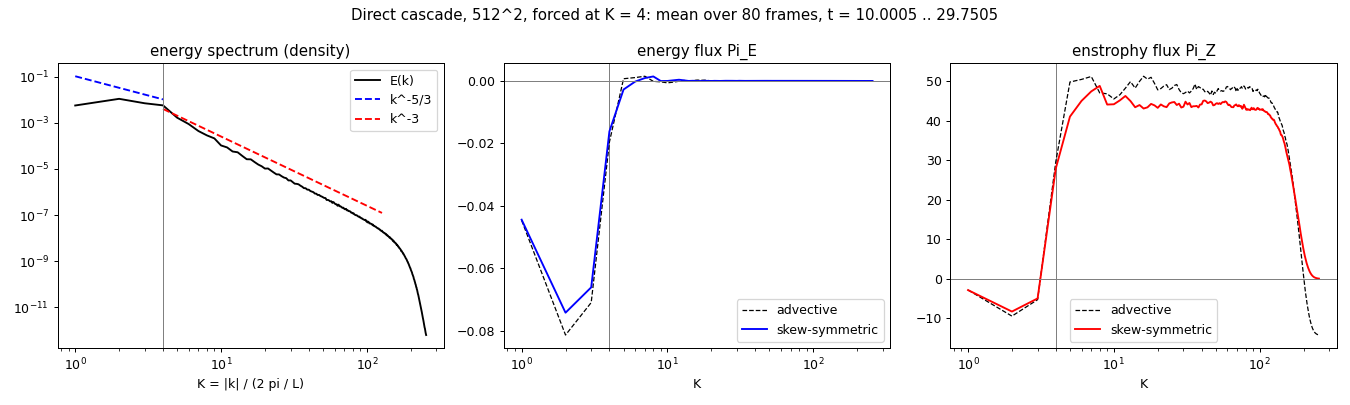
\includegraphics[width=\textwidth]{cascade_direct.png}
\caption{Direct cascade: time-mean energy spectrum (with $k^{-5/3}$ and $k^{-3}$ for reference) and fluxes, skew-symmetric form; dashed, the advective form.}
\label{fig:direct}
\end{figure}

\paragraph{Inverse cascade.}  $\Pi_E$ lies between $-0.093$ and $-0.096$, about $-0.95\,\varepsilon$, over $K=20$--$38$ (\cref{fig:inverse}), and $k^{5/3}E(k)$ is flat to $\pm6\,\%$ over $K=12$--$30$.  The hypodrag, whose rate is $\alpha_h/k^2$, takes the energy out over $K\approx2$--$15$, which ends the plateau there.  The hypodrag removes $0.093$ and the hyperviscosity $0.004$, and the nonlinear term $0.001$, $3\,\%$ short of $\varepsilon=0.1$.  The difference is a secular drift, not noise: $E$ still rises from $0.152$ to $0.170$ over the window, $\mathrm{d}E/\mathrm{d}t=+0.0023$, so the state is close to stationary but not exactly.  With the drift the implied input is $0.1005$, within $0.5\,\%$ of $\varepsilon$ ($0.7$ standard errors).  With $M=248$ forced modes the realized input scatters by only $0.0006$, unlike the direct run.  Over 400 frames $\Pi_E$ stays within $-0.0912$ to $-0.0951$ on $K=20$--$38$ (spread $4\,\%$).  Above the forcing the enstrophy flux is $5.8$--$5.9\times10^3$ over $K=42$--$100$, and the net enstrophy transfer is $10^{-13}$.  With the advective form the nonlinear term creates $2.85\times10^3$ per unit time near the cutoff, $45\,\%$ of the input; the hyperviscosity then removes $8.8\times10^3$ instead of $5.9\times10^3$.  The implied Kolmogorov constant, $k^{5/3}E/|\Pi_E|^{2/3}\approx9$, is above the $\approx6$ of well-resolved studies \cite{boffetta2012}, which is not surprising for an inertial range of a factor of 2.5 squeezed between the forcing and the hypodrag.

\begin{figure}[htbp]
\centering
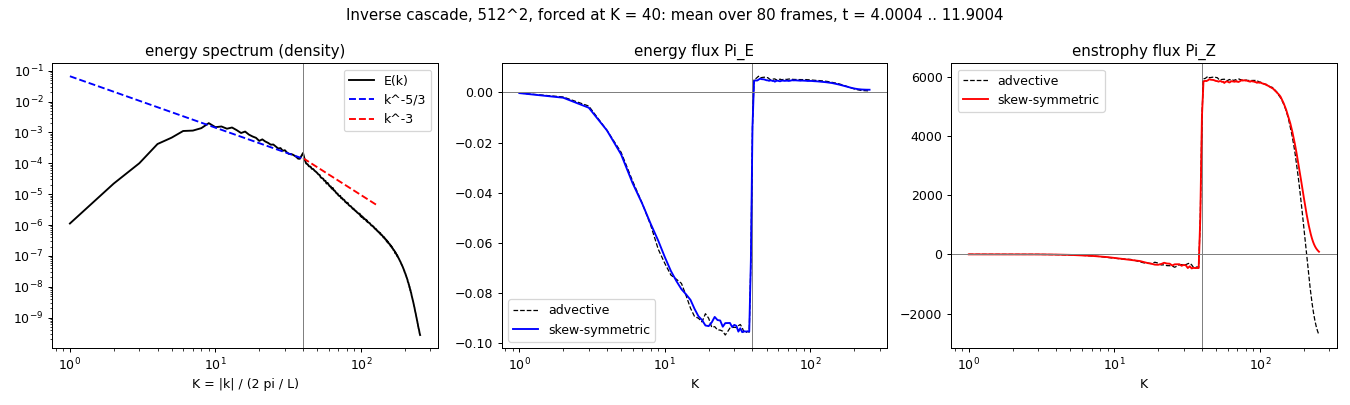
\includegraphics[width=\textwidth]{cascade_inverse.png}
\caption{Inverse cascade: as \cref{fig:direct}, forced at $K=40$.}
\label{fig:inverse}
\end{figure}

\paragraph{Decaying turbulence.}  \code{--case decaying} starts from random phases with modal amplitudes of envelope $E(k)\propto(k/k_0)^4e^{-2(k/k_0)^2}$ and $E=\tfrac12$ (\cref{sec:periodic}).  On $512^2$ with $k_0=10$, the hyperviscosity of the direct run ($\nu_h=10^{-23}$, $p=4$), $\Rey=10^7$ and the skew-symmetric form, run to $t=20$ (50\,000 steps), $E$ falls by $0.6\,\%$ while $Z$ falls by a factor of 15, as it should at high Reynolds number: the direct cascade carries enstrophy to the cutoff, where it is dissipated, and energy goes to large scales, where nothing removes it (\cref{fig:decaying}).  The peak of the spectrum moves from $K=9$ to $K=1$, which holds $59\,\%$ of the energy at the end.  Isolated coherent vortices emerge and merge \cite{mcwilliams1984}, and $Z$ drops in steps at the mergers.

\begin{figure}[htbp]
\centering
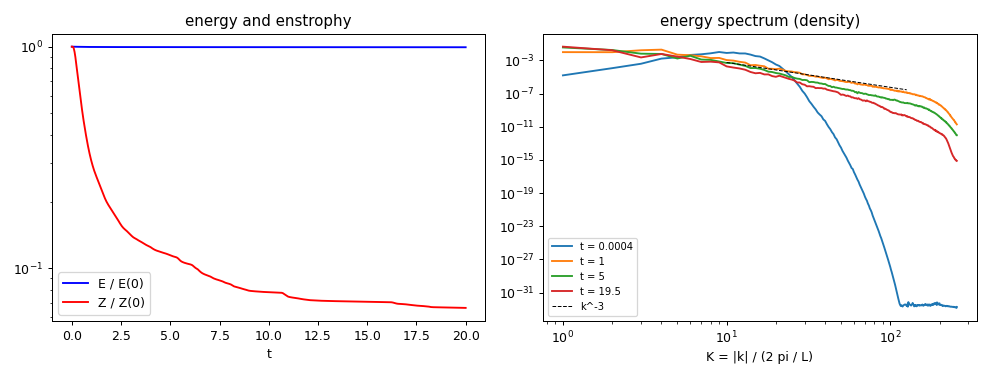
\includegraphics[width=0.9\textwidth]{decaying.png}\\[1ex]
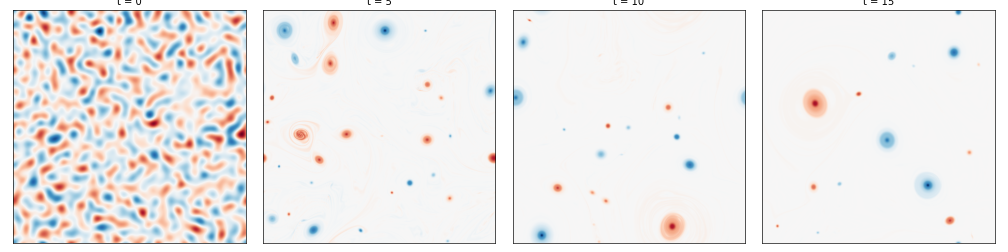
\includegraphics[width=\textwidth]{decaying_vortices.png}
\caption{Decaying turbulence on $512^2$: energy and enstrophy, energy spectra, and the vorticity at $t=0$, 5, 10 and 15.}
\label{fig:decaying}
\end{figure}

\paragraph{Resolution.}  How much of the spectrum does each order resolve?  Decaying turbulence at $\Rey=2\times10^4$ (skew-symmetric form, $k_0=10$) was run on $256^2$ and $512^2$ with orders 2, 4 and 6 and the compact scheme of \cref{sec:compact}, and on $2048^2$ with order 6, all with the same time step ($6.25\times10^{-5}$) and from the same initial field: the phases of the initial spectrum depend on the wavevector only, so every grid that resolves the spectrum gets the same field (\code{random\_initial\_field()}; \code{make test} checks it to $3\times10^{-16}$).  Turbulence is chaotic, so the runs decorrelate.  At $t=0.5$ the shell energies differ by tens of per cent even at $K=10$.  At $t=0.09$, about six eddy turnovers, after the cascade has filled the spectrum, the large scales ($K\le20$) of the $512^2$ runs still agree with the $2048^2$ one to $2\times10^{-4}$ (order 6) and $6\times10^{-5}$ (compact).  A common time step matters here: an earlier comparison with a reference whose frames fell half a step later agreed only to $2\times10^{-3}$.  The spectra are compared there (\cref{fig:resolution}); the reference is resolved, with $E$ at $K=256$ at $10^{-8}$ of its peak, and order 6 on $2048^2$ differentiates that shell to $0.2\,\%$:
\begin{center}\small
\setlength{\tabcolsep}{4pt}
\begin{tabular}{lccccccc}
\toprule
to $10\,\%$ ($2\,\%$) up to $K=$ & spectral & spectral, 3/2 & spectral, 2/3 & compact 6 & order 6 & order 4 & order 2 \\
\midrule
$512^2$ ($K_{\mathrm{Nyq}}=255$) & 235 (201) & 239 (198) & 143 (103) & 198 (167) & 152 (111) & 133 (73) & 60 (28) \\
$256^2$ ($K_{\mathrm{Nyq}}=127$) & 93 (57) & 93 (61) & 50 (29) & 118 (67) & 74 (48) & 60 (30) & 29 (1) \\
\bottomrule
\end{tabular}
\end{center}
Orders 6, 4 and 2 resolve the spectrum to $10\,\%$ up to about $59$, $49$ and $23\,\%$ of the Nyquist wavenumber, and to $2\,\%$ up to $38$--$44$, $24$--$29$ and at most $11\,\%$.  The compact scheme resolves $78$--$93\,\%$ to $10\,\%$ and $53$--$65\,\%$ to $2\,\%$: 1.3--1.6 times as many shells as explicit order 6 on the same grid, in line with its modified wavenumber (\cref{sec:compact}).  Beyond that the finite differences underestimate the derivatives, and the spectrum falls below the reference; the compact scheme on $256^2$ first overshoots it, by up to $8\,\%$ around $0.85\,K_{\mathrm{Nyq}}$.  Order 6 on $256^2$ resolves more shells than order 2 on $512^2$, at about half the cost per step ($3.3$ against $5.6\,\mathrm{ms}$ on the GPU).  In its banded form the compact scheme costs 20 times explicit order 6 per step, so it does not pay; in Fourier space (\cref{sec:fourier-ops}) it costs $1.3$--$1.4$ times.

Pseudospectral differentiation (\cref{sec:fourier-ops}) resolves the most on $512^2$, where the spectrum has fallen to $10^{-8}$ of its peak at the Nyquist wavenumber: $92\,\%$ of the range to $10\,\%$ and $79\,\%$ to $2\,\%$.  On $256^2$, where it is still at $10^{-6}$, it resolves less than the compact scheme.  Nothing damps the modes near the cutoff, so energy piles up there, up to twice the reference at the Nyquist wavenumber (\cref{fig:resolution-fourier}).  Aliasing does not explain it: with $3/2$ padding, which removes the quadratic aliasing from every mode but the Nyquist ones, the range is the same ($239$ and $93$ shells) and so is the pile-up ($1.8$ and $2.2$ times the reference).  This is consistent with an accumulation caused by the truncation itself: the enstrophy the cascade carries to the cutoff is not dissipated fast enough before it, as in Galerkin-truncated flows \cite{frisch2008}.  These runs rule out aliasing; they do not by themselves identify the mechanism.  The finite differences underestimate the derivatives there instead, and their spectra fall below the reference.  The 2/3 rule caps the range at $2/3$ of the Nyquist wavenumber by construction, and the energy piles up below that cutoff, which nothing dissipates either.  It resolves $56\,\%$ ($512^2$) and $39\,\%$ ($256^2$) to $10\,\%$, less than undealiased spectral and than compact.  Its merit is exact conservation, not resolution.

What a resolved shell costs follows from the step time and the advective limit.  Explicit time steps go as $h/(k^*h)_{\max}$: $1.59$ for order 6, $1.99$ compact, $\pi$ spectral (padded or not), and $2\pi/3$ with the 2/3 rule.  So the cost per unit simulated time at the advective limit is proportional to (ms per step)$\times(k^*h)_{\max}$.  The resolved range of explicit order 6 grows linearly with $n$ (74 on $256^2$, 152 on $512^2$), and its cost per unit time as $n^3$.  To resolve on its own grid what compact resolves on $512^2$ it needs $(198/152)^3=2.2$ times its $512^2$ cost, $45$ against the compact $35$ (in ms per step times $(k^*h)_{\max}$): compact is $22\,\%$ cheaper.  Pseudospectral is $26\,\%$ cheaper ($56$ against $75$).  On $256^2$ compact is $2.4$ times cheaper ($9.5$ against $23$), and undealiased spectral is $34\,\%$ dearer ($15.1$ against $11.3$).  Padding costs $1.85$ times per step ($31.4$ against $17.0\,\mathrm{ms}$ on $512^2$, $7.8$ against $4.7$ on $256^2$, five transforms on $(3n/2)^2$ points against three on $n^2$), for the same range: padded pseudospectral costs $1.3$ ($512^2$) and $2.3$ ($256^2$) times explicit order 6 at equal range.  These gains are modest where the flow is resolved, and depend on how close to the cutoff the spectrum carries energy.  In the tested decaying runs (one Reynolds number, one initial spectrum, two grids), compact sixth-order differentiation gave the most robust cost--resolution trade-off.  Pseudospectral differentiation became advantageous once the grid resolved the high-wavenumber tail.  The 2/3 rule trades a third of the range for exact conservation.  The next paragraphs test whether this ordering holds at other Reynolds numbers, for other spectra and in forced turbulence.

\begin{figure}[htbp]
\centering
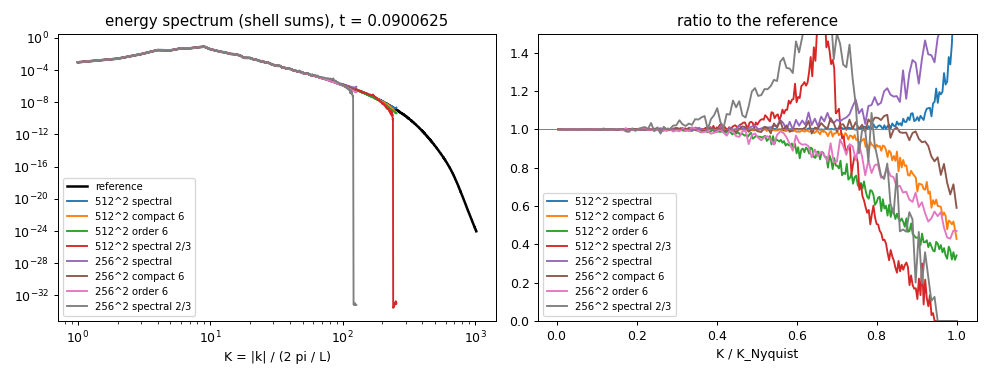
\includegraphics[width=0.9\textwidth]{resolution_fourier.png}
\caption{As \cref{fig:resolution}, with pseudospectral differentiation, with and without the 2/3 rule.}
\label{fig:resolution-fourier}
\end{figure}

\paragraph{Does the ordering hold across regimes?}  The comparison above is one flow: decaying turbulence at $\Rey=2\times10^4$ from $k_0=10$.  To see whether its ordering is robust, the same comparison was repeated varying one parameter at a time: $\Rey=5\times10^3$ and $8\times10^4$, and $k_0=5$ and $20$, each on $256^2$ and $512^2$ against its own $2048^2$ reference.  The comparison time keeps $t/\tau_0$ fixed, $\tau_0\propto1/k_0$ (all runs start with $E=\tfrac12$): $t=0.09\cdot10/k_0$, about six eddy turnovers.  The largest scales ($K\le20$) still agree with the reference to $10^{-3}$--$10^{-2}$ there, so the comparison is made before the runs decorrelate.  A $2048^2$ explicit-order-6 run is taken as the reference only where it does not depend on its own discretization.  For the two most demanding cases ($\Rey=8\times10^4$, $k_0=20$) a second, independent $2048^2$ run with the compact scheme agrees with it to $1.5\times10^{-3}$ up to $K=255$ (and to $10^{-4}$ up to $K=127$), well inside the $2\,\%$ and $10\,\%$ tolerances measured; the two differ only beyond $K\approx500$, the upper half of their own range.  The question is whether a single parameter, the reference's energy at the grid's Nyquist shell relative to its peak, $E(K_{\mathrm{Nyq}})/E_{\max}$, orders the schemes.  It measures how much of the flow lies at the cutoff.  The scripts are \code{tools/compare\_schemes.py} (per case and the plot of \cref{fig:crossover}).

\begin{center}\small
\setlength{\tabcolsep}{4pt}
\begin{tabular}{llccccccc}
\toprule
case & grid & $E(K_{\mathrm{Nyq}})/E_{\max}$ & order 6 & compact 6 & spectral & spectral, 3/2 & spectral, 2/3 \\
\midrule
$\Rey=5\times10^3$ & $512^2$ & $2.8\times10^{-12}$ & 144 & 196 & \textbf{249} & 248 & 163 \\
$k_0=5$ & $512^2$ & $4.2\times10^{-11}$ & 146 & 197 & \textbf{246} & \textbf{246} & 154 \\
baseline & $512^2$ & $1.5\times10^{-8}$ & 152 & 198 & 235 & \textbf{239} & 143 \\
$k_0=5$ & $256^2$ & $9.0\times10^{-8}$ & 71 & 105 & 101 & \textbf{109} & 62 \\
$\Rey=5\times10^3$ & $256^2$ & $2.0\times10^{-7}$ & 74 & 105 & \textbf{120} & \textbf{120} & 70 \\
$\Rey=8\times10^4$ & $512^2$ & $2.3\times10^{-7}$ & 152 & \textbf{217} & 193 & 200 & 117 \\
$k_0=20$ & $512^2$ & $1.6\times10^{-6}$ & 159 & 213 & \textbf{217} & \textbf{217} & 130 \\
baseline & $256^2$ & $4.9\times10^{-6}$ & 74 & \textbf{118} & 93 & 93 & 50 \\
$\Rey=8\times10^4$ & $256^2$ & $1.2\times10^{-5}$ & \textbf{80} & 79 & 75 & 79 & 46 \\
$k_0=20$ & $256^2$ & $1.6\times10^{-4}$ & \textbf{89} & 74 & 74 & 72 & 49 \\
\bottomrule
\end{tabular}
\end{center}
(shells within $10\,\%$ of the reference).  In these decaying runs, before decorrelation, the parameter largely organizes the ordering (\cref{fig:crossover}).  Relative to explicit order 6, pseudospectral differentiation resolves $1.7$ times as many shells where the cutoff carries $10^{-11}$ of the peak, and falls steadily to $0.83$ at $10^{-4}$.  The compact scheme stays at $1.3$--$1.6$ times up to about $5\times10^{-6}$ and then drops to parity and below.  The 2/3 rule falls monotonically from $1.13$ to $0.55$.  $3/2$ padding follows undealiased spectral within $8$ shells in every case (the open diamonds of \cref{fig:crossover}); it moves the crossover with compact by at most one case ($k_0=5$ on $256^2$, $109$ against $105$).  Pseudospectral is ahead below about $10^{-7}$.  Above about $10^{-5}$ neither high-resolution scheme beats explicit order 6, whose underestimated derivatives near the cutoff behave like a numerical damping there.  The crossover between compact and pseudospectral lies between $10^{-7}$ and $10^{-6}$ and is not sharp.  At $2.0$ and $2.3\times10^{-7}$ the two cases come out in opposite order, so near the crossover something besides the energy at the cutoff decides.  A second parameter, presumably the spectral slope at the cutoff, $\mathrm{d}\log E/\mathrm{d}\log k$ at $K_{\mathrm{Nyq}}$, may complete the description; that was not tested.

The cost at equal resolved range, relative to explicit order 6 as in \cref{sec:fourier-ops}, follows the same axis.  Compact costs $0.57$--$0.78$ times wherever $E(K_{\mathrm{Nyq}})/E_{\max}\lesssim5\times10^{-6}$.  Pseudospectral costs $0.54$--$0.74$ times only below about $10^{-8}$, and $1.0$--$1.4$ around the crossover.  In the heavily under-resolved cases ($\gtrsim10^{-5}$) both cost more (compact $1.9$--$3.1$, pseudospectral $3.4$--$4.9$).  The 2/3 rule never costs less ($1.3$--$11$), and neither does $3/2$ padding: at the same range as undealiased spectral and $1.85$ times its step, it costs $1.00$--$1.31$ times explicit order 6 where pseudospectral leads, and $2$--$9$ times in the under-resolved cases.

In forced turbulence the runs decorrelate, so the comparison is between time-mean statistics, and those carry the sampling scatter of the random forcing.  With 28 forced modes, the realized enstrophy input over the averaging windows used here varies by about $\pm8\,\%$.  This sets a floor below which the schemes cannot be told apart.  The forced direct cascade with hyperviscosity (\cref{sec:cascade}, $256^2$, $t=6$--$16$) gives the same slope with all four ($-3.44$ to $-3.48$), and the enstrophy flux leaves its plateau at the same $K=66$, where the hyperviscosity takes over.  The plateau levels ($41.9$, $43.0$, $46.2$, $50.1$ for order 6, compact, spectral, spectral 2/3) differ as much as the total enstrophy each run removed, so they reflect the realized input, not the cascade.  Three are within one standard deviation and the dealiased run within about two.  With the dissipation confined near the cutoff, the scheme makes no measurable difference here.

With plain viscosity ($\Rey=10^5$, hypodrag, no hyperviscosity, $256^2$, $t=4$--$10$) the dissipation range is resolved by the flow itself, not by the grid.  The reference is a $768^2$ pseudospectral run, whose energy at its own Nyquist shell is $1.4\times10^{-11}$ of the peak; at the $256^2$ cutoff the energy is $2.8\times10^{-7}$ of the peak, near the decaying crossover.  Normalising each spectrum by its own enstrophy flux, $E\propto\Pi_Z^{2/3}$, takes out the realized input.  The spectra then agree with the reference to $10\,\%$ from $K=8$ up to $K=100$ (order 6), $89$ (spectral), $84$ (compact) and $42$ (spectral, 2/3).  At this cutoff energy the decaying cases put pseudospectral or compact ahead; here explicit order 6 holds the longest.  The differences are within the remaining scatter, though: away from the cutoff the normalised spectra still differ from the reference by up to $8\,\%$.  What does stand out is how each scheme behaves at the cutoff.  At $K=120$, order 6 is low ($0.64$ of the reference) and pseudospectral piles energy up ($1.53$, and $2.0$ at the Nyquist shell).  Compact is in between ($1.00$, overshooting by up to $17\,\%$ just below), and the 2/3 rule truncates.  So the energy at the cutoff is a useful organizing parameter for transient decaying turbulence, not a universal predictor of how the schemes rank.  In these forced cases the schemes are not distinguishable in the inertial range, and they differ at the cutoff in the characteristic ways seen throughout: explicit stencils fall below the reference, pseudospectral piles up, compact lies between.

\begin{figure}[htbp]
\centering
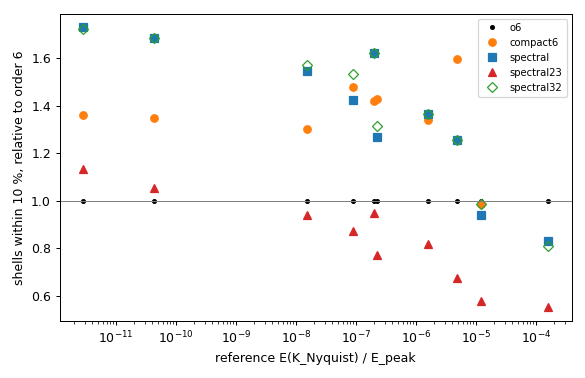
\includegraphics[width=0.7\textwidth]{crossover.png}
\caption{Shells within $10\,\%$ of the reference, relative to explicit order 6, against the reference's energy at the grid's Nyquist shell relative to its peak: five decaying cases ($\Rey$ and $k_0$ varied about the baseline) on $256^2$ and $512^2$.  Open diamonds: pseudospectral with $3/2$ padding, on top of the undealiased squares.}
\label{fig:crossover}
\end{figure}

\paragraph{Compact schemes in forced turbulence.}  The direct-cascade run on $256^2$, with the hyperviscosity scaled to that grid ($\nu_h=1.66\times10^{-21}$, $p=4$), the same seed and time step and averaged over $t=6$--$16$, gives nearly the same statistics with both schemes (\cref{fig:compact-turbulence}).  The enstrophy-flux plateau over $K=8$--$50$ is $41.9$ (spread $5\,\%$) with order 6 and $42.9$ ($3\,\%$) compact, and the spectral slope there is $-3.44$ and $-3.48$.  The flux falls below $90\,\%$ of the plateau at $K=66$ in both, where the hyperviscosity takes over.  Over $K=20$--$60$ the two spectra agree to $1$--$2\,\%$; above $K\approx80$ the compact run carries $8$--$25\,\%$ more energy.  That is where the first derivative of order 6 is off by more than $10\,\%$ ($K/K_{\mathrm{Nyq}}>0.54$).  With the dissipation confined to that range, the scheme changes the dissipation range and not the inertial one, at 15 times the cost per step in its banded form ($66$ against $4.4\,\mathrm{ms}$), about 1.4 times in Fourier space.  The compact scheme pays off where a flow needs accurate derivatives close to the grid cutoff, as in the decaying runs above, and not in this set-up.

\begin{figure}[htbp]
\centering
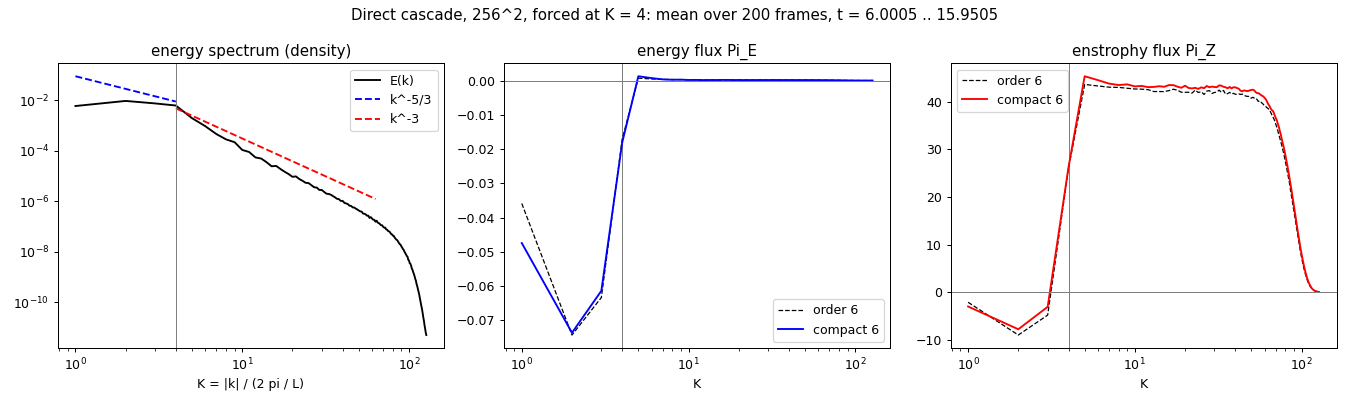
\includegraphics[width=\textwidth]{cascade_compact.png}
\caption{Direct cascade on $256^2$ with the compact scheme: time-mean spectrum and fluxes; dashed, explicit order 6.}
\label{fig:compact-turbulence}
\end{figure}

\begin{figure}[htbp]
\centering
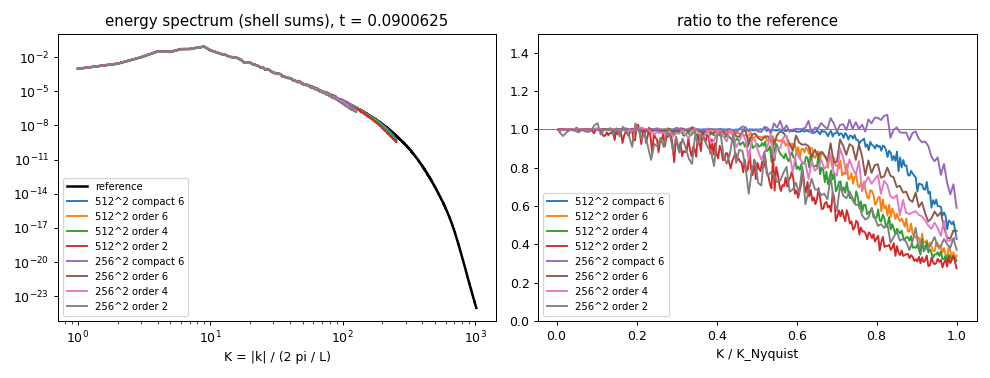
\includegraphics[width=0.9\textwidth]{resolution.png}
\caption{Decaying turbulence at $t=0.09$: energy spectra of $256^2$ and $512^2$ runs with orders 2, 4 and 6 and the compact scheme, and their ratio to a $2048^2$ order-6 run.}
\label{fig:resolution}
\end{figure}

\subsection{Physical validation against Ghia et al.}
\label{sec:ghia}

The code embeds the standard $\Rey=100$ centerline velocity values from Ghia et al. \cite{ghia1982} and writes them alongside the simulation profile.  This supports a conventional cavity-flow validation workflow:
\begin{enumerate}[leftmargin=2em]
  \item run to a demonstrably steady state;
  \item interpolate the numerical centerline velocity to the Ghia sample coordinates, or vice versa;
  \item compute $L_2$, $L_\infty$, and selected pointwise errors;
  \item repeat on successively refined grids;
  \item repeat with smaller timesteps to separate spatial and temporal error.
\end{enumerate}

For the default case ($\Rey=100$, RK4, FFT solver, $t_f=30$), the simulated centerline velocities interpolated to the 15 interior Ghia points give:

\begin{center}
\begin{tabular}{lcccc}
\toprule
 & \multicolumn{2}{c}{$u$ on $x=0.5$} & \multicolumn{2}{c}{$v$ on $y=0.5$} \\
Grid & max error & rms error & max error & rms error \\
\midrule
$64\times64$, mixed convention (before) & 0.0594 & 0.0372 & 0.0595 & 0.0301 \\
$64\times64$, nodal convention & 0.0023 & 0.0014 & 0.0073 & 0.0039 \\
$65\times65$, nodal convention & 0.0026 & 0.0014 & 0.0076 & 0.0039 \\
$129\times129$, nodal convention & 0.0045 & 0.0024 & 0.0089 & 0.0049 \\
$257\times257$, nodal convention & 0.0050 & 0.0025 & 0.0091 & 0.0051 \\
\bottomrule
\end{tabular}
\end{center}

The solution has converged at these resolutions: at the Ghia points the $129\times129$ and $257\times257$ profiles differ by at most $4.5\times10^{-4}$ ($u$) and $3.5\times10^{-4}$ ($v$), an order of magnitude less than either differs from the reference.  The remaining discrepancy is therefore not grid error of this code; it is of the order of the accuracy of the reference data themselves, which were computed on a $129\times129$ grid with a second-order scheme.  The errors grow slightly from $64\times64$ to $129\times129$: the smaller error of the coarse grid comes partly from its discretisation error cancelling against the difference to the reference, so $64\times64$ should not be read as the most accurate grid.  The $257\times257$ run used $\dt=3\times10^{-4}$.

\code{make regression} automates this comparison for the default case: the steady centerline profiles must be within $0.004$ ($u$) and $0.010$ ($v$) of the reference values, which are stored with the tests rather than taken from the program's output, and any value that is not a finite number fails.  Grid-convergence rates are not measured on the cavity, for the reason given in \cref{sec:mms}, but on a manufactured solution.

% =============================================================================
\section{Performance Characteristics}
% =============================================================================

The default FFT-based Poisson solver generally dominates the timestep cost, especially under RK4 where five elliptic solves are performed per step.  Measured timings per timestep for the CPU, OpenMP and CUDA builds are kept in one place, the Performance section of \code{README.md}, so that they are not maintained in two copies; they are implementation benchmarks on one machine rather than performance guarantees.

For transform performance, grid sizes for which $n-1$ factors into small primes are advantageous, because the sine transform of the $n-2$ interior nodes acts through FFT lengths of $2(n-1)$.  Sizes such as 65, 129, 257, 513 and 1025 are therefore fast, and their neighbours can be several times slower: on the machine of the README benchmarks one serial FFT Poisson solve takes 6.7\,ms at $255^2$ ($2(n-1)=508=4\cdot127$) against 1.6\,ms at $257^2$ ($512$), and 85\,ms at $1023^2$ against 31\,ms at $1025^2$.

The GPU becomes increasingly advantageous as the grid grows because the fixed kernel-launch overhead is amortized over more work.  Double-precision FFT throughput is a major cost on consumer GPUs, so larger speedups may be observed on hardware with stronger FP64 capability.

% =============================================================================
\section{Building and Running}
% =============================================================================

\subsection{Dependencies}

The CPU solver requires a C compiler, the math library, and FFTW3.  OpenMP is optional.  CUDA requires the NVIDIA CUDA toolkit and cuFFT.

On Ubuntu/Debian, a typical CPU setup is
\begin{lstlisting}[language=bash]
sudo apt install build-essential libfftw3-dev
\end{lstlisting}
For CUDA development, the distribution toolkit or NVIDIA's toolkit packages may be used.

\subsection{Build modes}

\begin{lstlisting}[language=bash]
make                    # serial CPU
make OPENMP=1           # OpenMP CPU
make CUDA=1             # CUDA-enabled binary
make OPENMP=1 CUDA=1    # CUDA plus OpenMP CPU fallback/tests
\end{lstlisting}

The Makefile records the active compiler flags so that changing OpenMP/CUDA modes triggers the required rebuild automatically.

\subsection{Tests}

\begin{lstlisting}[language=bash]
make test
make CUDA=1 test
make OPENMP=1 CUDA=1 test
make OPENMP=1 convergence   # spatial convergence study, about 1.5 minutes
\end{lstlisting}

The test program returns 0 when all executed checks pass, 1 when any check fails, and 77 when a CUDA test build cannot execute its GPU checks because no usable device is present.

Further checks, each a \code{make} target run by continuous integration: \code{test-cli} (invalid command lines are refused, with the program's error status and message, without writing anything), \code{regression} (a short run against stored results and the steady default case against Ghia et al.), \code{test-asan} (AddressSanitizer and UndefinedBehaviorSanitizer), \code{valgrind} (no leaks, nothing still reachable), \code{format-check}, \code{cppcheck}, \code{tidy} (also over the CUDA and OpenMP branches of the C sources; the CUDA source itself is checked only by its compiler), and \code{WERROR=1} builds, which make nvcc's warnings errors too.  Continuous integration has no GPU, so the CPU--GPU comparisons run only where \code{make CUDA=1 test} is run on a GPU host.

\subsection{Runtime options}

The current binary accepts:

\begin{longtable}{@{}>{\ttfamily}p{0.30\textwidth}p{0.62\textwidth}@{}}
\toprule
\normalfont Option & Description \\
\midrule
\endhead
--nx N & Number of grid points in $x$. \\
--ny N & Number of grid points in $y$. \\
--n N & Same number of grid points in $x$ and $y$. \\
--dt DT & Timestep. \\
--tf TF & Final simulation time. \\
--output-interval N & Write VTK every $N$ steps; zero disables VTK output. \\
--re RE & Reynolds number. \\
--poisson-order N & 2 (five-point, default) or 4 (compact, \cref{sec:compact-poisson}); FFT solver with walls. \\
--wall-closure NAME & \texttt{velocity} (default) or \texttt{briley} (\cref{eq:briley}). \\
--velocity-order N & 2 (default) or 4: fourth-order rows next to the walls for $u$, $v$ (\cref{sec:wall-order}). \\
--integrals-interval N & Write $E$, $Z$, $P$, $I$ to \texttt{output/integrals.csv} every $N$ steps (default 1; 0 never; \cref{sec:diagnostics}). \\
--drag A & Periodic cases: linear drag $-\alpha\omega$ (\cref{sec:forcing}). \\
--kolmogorov-amp A & Periodic cases: Kolmogorov forcing amplitude; \texttt{--kolmogorov-n} its wavenumber. \\
--forcing-rate EPS & Periodic cases: random forcing rate; \texttt{--forcing-k}, \texttt{--forcing-width} its shell, \texttt{--seed} its seed. \\
--hyperviscosity NU & Periodic cases: hyperviscosity $\nu_h$; \texttt{--hyper-order} its order $p$ (default 4). \\
--hypodrag A & Periodic cases: hypodrag $\alpha_h$ (\cref{sec:forcing}). \\
--advection NAME & Periodic cases: \texttt{advective} or \texttt{skew} nonlinear term (\cref{eq:skew}); default \texttt{skew} for \texttt{forced} and \texttt{decaying}. \\
--spectrum-interval N & Periodic cases: write the spectra every $N$ steps (default: with the VTK frames). \\
--peak-k K0 & \texttt{decaying}: peak of the initial spectrum. \\
--case NAME & \texttt{cavity} (default), or on a doubly periodic unit square \texttt{taylor-green}, \texttt{shear-layer}, \texttt{kolmogorov}, \texttt{forced} or \texttt{decaying} (\cref{sec:periodic,sec:forcing}). \\
--cpu & In a CUDA build, force the CPU backend. \\
--help & Print command-line help. \\
\bottomrule
\end{longtable}

Example:
\begin{lstlisting}[language=bash]
mkdir -p output
./cnavier --n 127 --dt 6.2e-4 --tf 20 --output-interval 50
\end{lstlisting}

Parameters such as Reynolds number, finite-difference order, Poisson method, and time integrator are presently configured in \code{src/main.c} rather than through command-line flags.

% =============================================================================
\section{Default Numerical Configuration}
% =============================================================================

At the repository state documented here, the source defaults are summarized in \cref{tab:defaults}.

\begin{table}[htbp]
\centering
\caption{Principal defaults in \code{src/main.c}.}
\label{tab:defaults}
\begin{tabular}{@{}lll@{}}
\toprule
Quantity & Default & Meaning \\
\midrule
$\Rey$ & 100 & Reynolds number \\
$L_x,L_y$ & 1, 1 & domain lengths \\
$n_x,n_y$ & 64, 64 & computational array size \\
$\dt$ & 0.005 & timestep \\
$t_f$ & 30 & final time \\
finite-difference \code{order} & 6 & sixth-order interior stencil \\
\code{time\_scheme} & 2 & classical RK4 \\
\code{poisson\_type} & 3 & FFT/DST-I direct discrete solver \\
Poisson iterate tolerance & $10^{-3}$ & GS/SOR iterate-change threshold \\
Poisson max iterations & 10000 & GS/SOR iteration cap \\
VTK output interval & 20 & steps between output files \\
\bottomrule
\end{tabular}
\end{table}

% =============================================================================
\section{Numerical Interpretation and Current Limitations}
% =============================================================================

The following points are important when interpreting results scientifically.

\subsection{Mixed formal spatial order}

The transport derivatives may be sixth-order in the deep interior, but the boundary closures are lower order and the Poisson solve is based on a second-order discrete Laplacian.  Measured against a smooth manufactured solution with stationary no-slip walls, the complete algorithm converges at second order in space for every derivative order, and orders 4 and 6 give the same errors (\cref{sec:mms}).  This is evidence for one solution family, not a proof for every flow.  The ablation of \cref{sec:ablation} shows that the Poisson operator and the wall-vorticity closure each limit the order to two on their own, so higher-order results need both improved; with the compact Poisson operator and the third-order wall closure (\cref{sec:wall-order}) the method reaches fourth order for $\omega$ and $\psi$, and with fourth-order velocity rows next to the walls for the velocity too.  Beyond fourth order, the transport operators' rows next to the walls would have to be raised as well.  On a doubly periodic grid, with no walls and a Poisson operator of the same order as the derivatives, the method reaches the nominal order 2, 4 or 6 (\cref{sec:periodic-verification}).

\subsection{Poisson operator differs from transport Laplacian}

The diffusion term in \cref{eq:vort-transport} uses the selected $D_{xx}+D_{yy}$ operator, while the streamfunction equation always uses the standard five-point second-order Laplacian.  This is a legitimate mixed discretization, but it should be described explicitly because the \code{order} setting does not uniformly change every spatial operator in the solver.

\subsection{Boundary vorticity accuracy}

Wall vorticity is reconstructed from differentiated wall velocities rather than from a dedicated high-order streamfunction wall formula.  Its accuracy is therefore tied to the one-sided derivative closure and the array-edge interpretation.

\subsection{Explicit stability}

At startup a lid-speed Courant check and the viscous bound of the selected time integrator (computed from the assembled second-derivative operator, so it follows the grid, Reynolds number and finite-difference order) are enforced.  These are stability bounds only; they say nothing about temporal accuracy, and users remain responsible for timestep-convergence studies.

\subsection{Steady-state convergence}

The default driver advances to a specified final time; it does not terminate based on a physical steady-state residual such as $\|\omega^{n+1}-\omega^n\|$ or a momentum residual.  For steady cavity studies, $t_f$ should be selected after checking that monitored fields and centerline profiles no longer change materially.

\subsection{Pressure is not solved}

Pressure is absent from the vorticity--streamfunction formulation.  This is an advantage for the cavity velocity field but means that pressure output is not currently a native solved quantity.  If pressure is required, it must be reconstructed from an additional pressure-Poisson or momentum-based relation with suitable boundary conditions.

\subsection{Geometry and dimensionality}

The current method is two-dimensional and Cartesian.  Curvilinear grids, immersed boundaries, unstructured meshes, three-dimensional vorticity stretching, and general inflow/outflow boundaries are outside the present scope.

% =============================================================================
\section{Suggested Scientific Workflow}
% =============================================================================

For a reproducible numerical experiment, the following workflow is recommended:

\begin{enumerate}[leftmargin=2em]
  \item Record the Git commit, compiler, optimization flags, FFTW/CUDA versions, CPU/GPU, and runtime backend.
  \item Run \code{make test} for the chosen CPU build; for CUDA work, also run the GPU comparison suite on the actual GPU host.
  \item Select a baseline grid and timestep conservatively.
  \item Confirm temporal convergence by reducing $\dt$ while holding the grid fixed.
  \item Confirm spatial convergence with at least three grids while keeping temporal error smaller than spatial error.
  \item For the lid-driven cavity, compare centerline profiles against Ghia et al. and report interpolation/error norms.
  \item For steady solutions, verify that extending $t_f$ does not materially change the solution.
  \item Report the discrete divergence extrema as an implementation consistency diagnostic, but do not substitute them for solution-convergence metrics.
\end{enumerate}

% =============================================================================
\section{Possible Methodological Extensions}
% =============================================================================

The current architecture makes several research-oriented extensions relatively natural:

\begin{itemize}[leftmargin=2em]
  \item a consistent fourth- or sixth-order Poisson discretization, solved by an appropriate sparse/direct/iterative method;
  \item dedicated high-order wall-vorticity formulas;
  \item adaptive timestep selection from advective and diffusive spectral bounds;
  \item automated steady-state residual monitoring;
  \item automated Ghia interpolation and error norms in the test suite;
  \item grid-convergence-index (GCI) reporting;
  \item alternative convection schemes, such as upwind-biased, compact or WENO, and with walls a skew-symmetric form (on periodic grids it is available, \cref{eq:skew});
  \item multigrid for the Poisson equation when boundary conditions or geometries no longer permit a separable sine transform;
  \item pressure reconstruction as a post-processing step;
\end{itemize}

% =============================================================================
\section{Final Remarks}
% =============================================================================

\texttt{cnavier} implements a mathematically clean and computationally compact route to incompressible flow in two dimensions: evolve vorticity, invert a scalar Poisson equation, and differentiate a streamfunction to recover velocity.  The code is particularly transparent because the spatial derivatives are explicit finite-difference matrices, the two-dimensional operators are tensor products, and both CPU and GPU backends expose the same algorithmic sequence.

The strongest parts of the present methodology are the exact discrete streamfunction enforcement of incompressibility, the direct DST-based Poisson option, reusable sparse operators, RK4 stage consistency, and unusually thorough CPU--GPU equivalence tests for a compact CFD code.  The main scientific qualifications are equally clear: high-order accuracy applies primarily to interior transport derivatives; boundary closures are lower order; the streamfunction Poisson operator is second order; and quantitative benchmark/grid-convergence validation is not yet automated.

For educational CFD, numerical experimentation, backend comparisons, and as a foundation for further research-oriented development, these characteristics make the project both useful and unusually auditable.  For publication-quality quantitative claims, the next step is not to complicate the code immediately, but to formalize its grid convention and add systematic temporal/spatial convergence and benchmark-error measurements.

% =============================================================================
\appendix
\section{Mapping Between Equations and Source Code}
% =============================================================================

\begin{longtable}{@{}p{0.34\textwidth}p{0.58\textwidth}@{}}
\toprule
Mathematical operation & Main implementation location \\
\midrule
\endhead
First-derivative stencils & \code{SDiff1()} in \code{src/finitediff.c} \\
Second-derivative stencils & \code{SDiff2()} in \code{src/finitediff.c} \\
Kronecker operators & \code{skronecker()} in \code{src/linearalg.c}; assembly in \code{src/main.c} \\
CSR derivative evaluation & \code{spmv()} in \code{src/linearalg.c}; \code{spmv\_kernel} on CUDA \\
Wall velocity condition & \code{apply\_wall\_bc()} / \code{wall\_bc\_kernel} \\
Wall vorticity & \code{step()} / \code{vorticity\_bc\_kernel} \\
Vorticity RHS & \code{dwdt()}, \code{euler()} / \code{rhs\_kernel} \\
RK4 & \code{rk4()} / CUDA stage kernels in \code{gpu\_step()} \\
Gauss--Seidel & \code{poisson()} / \code{poisson\_redblack()} \\
SOR & \code{poisson\_SOR()} / \code{poisson\_redblack()} \\
FFT/DST-I Poisson & \code{poisson\_FFT()} / \code{poisson\_fft()} \\
Velocity recovery & \code{velocity\_from\_vorticity()} / \code{velocity\_kernel} \\
Divergence diagnostic & main-loop CSR operations / \code{continuity\_kernel} \\
Ghia centerlines & \code{print\_centerline()} in \code{src/utils.c} \\
Verification suite & \code{tests/test\_solver.c} \\
\bottomrule
\end{longtable}

% =============================================================================
\section{Reproducibility Record}
% =============================================================================

This document was prepared from the public repository
\begin{center}
\url{https://github.com/leo-aa88/cnavier}
\end{center}
with \code{main} observed at commit
\begin{center}
\code{5018e29bff534b252a7ac9025ece4ac43efd78ad}
\end{center}
on 6 October 2026.  Numerical details in this manual describe the source code at that repository state; later commits may change defaults or algorithms.

% =============================================================================
\begin{thebibliography}{9}

\bibitem{ghia1982}
U. Ghia, K. N. Ghia, and C. T. Shin,
``High-Re solutions for incompressible flow using the Navier--Stokes equations and a multigrid method,''
\emph{Journal of Computational Physics}, vol. 48, no. 3, pp. 387--411, 1982.

\bibitem{ferziger}
J. H. Ferziger, M. Peri\'{c}, and R. L. Street,
\emph{Computational Methods for Fluid Dynamics}, 4th ed., Springer, 2020.

\bibitem{leveque}
R. J. LeVeque,
\emph{Finite Difference Methods for Ordinary and Partial Differential Equations},
SIAM, 2007.

\bibitem{fftw}
M. Frigo and S. G. Johnson,
``The design and implementation of FFTW3,''
\emph{Proceedings of the IEEE}, vol. 93, no. 2, pp. 216--231, 2005.

\bibitem{lele1992}
S. K. Lele,
``Compact finite difference schemes with spectral-like resolution,''
\emph{Journal of Computational Physics}, vol. 103, no. 1, pp. 16--42, 1992.

\bibitem{kraichnan1967}
R. H. Kraichnan,
``Inertial ranges in two-dimensional turbulence,''
\emph{Physics of Fluids}, vol. 10, no. 7, pp. 1417--1423, 1967.

\bibitem{mcwilliams1984}
J. C. McWilliams,
``The emergence of isolated coherent vortices in turbulent flow,''
\emph{Journal of Fluid Mechanics}, vol. 146, pp. 21--43, 1984.

\bibitem{boffetta2012}
G. Boffetta and R. E. Ecke,
``Two-dimensional turbulence,''
\emph{Annual Review of Fluid Mechanics}, vol. 44, pp. 427--451, 2012.

\bibitem{frisch2008}
U. Frisch, S. Kurien, R. Pandit, W. Pauls, S. S. Ray, A. Wirth and J.-Z. Zhu,
``Hyperviscosity, Galerkin truncation, and bottlenecks in turbulence,''
\emph{Physical Review Letters}, vol. 101, p. 144501, 2008.

\bibitem{canuto2006}
C. Canuto, M. Y. Hussaini, A. Quarteroni and T. A. Zang,
\emph{Spectral Methods: Fundamentals in Single Domains}, Springer, 2006.

\end{thebibliography}

\end{document}
